\documentclass[hidelinks,onefignum,onetabnum,final]{siamart220329}  % for arxiv
%\documentclass[review,hidelinks,onefignum,onetabnum,final]{siamart220329}  % for submission

\usepackage{amsfonts,yhmath}
\usepackage{graphicx}
\usepackage{epstopdf}
\ifpdf
  \DeclareGraphicsExtensions{.eps,.pdf,.png,.jpg}
\else
  \DeclareGraphicsExtensions{.eps}
\fi

% Used for creating new theorem and remark environments
\newsiamremark{remark}{Remark}
\newsiamthm{claim}{Claim}
\newsiamremark{example}{Example}

\newcommand{\newindthm}[2]{
  \theoremstyle{plain}
  \theoremheaderfont{\normalfont\sc}
  \theorembodyfont{\normalfont\itshape}
  \theoremseparator{.}
  \theoremsymbol{}
  \newtheorem{#1}{#2}
}
\newindthm{conjecture}{Conjecture}
\renewcommand{\theconjecture}{\Alph{conjecture}}

\newcommand{\newindthmstar}[2]{
  \theoremstyle{plain}
  \theoremheaderfont{\normalfont\sc}
  \theorembodyfont{\normalfont\itshape}
  \theoremseparator{.}
  \theoremsymbol{}
  \newtheorem*{#1}{#2}
}
\newindthmstar{assumptions}{Standard Assumptions}

\usepackage{amsopn}
\DeclareMathOperator{\diag}{diag}

\usepackage{bm,bbm,empheq,verbatim,fancyvrb,amssymb}
\usepackage{booktabs,multirow,xspace}
\usepackage{pifont}

\usepackage{tikz}
%\usetikzlibrary{math}

\newcommand{\eps}{\epsilon}
\newcommand{\RR}{\mathbb{R}}

\newcommand{\grad}{\nabla}
\newcommand{\Div}{\nabla\cdot}

\newcommand{\bbf}{\mathbf{f}}
\newcommand{\bg}{\mathbf{g}}
\newcommand{\bn}{\mathbf{n}}
\newcommand{\bu}{\mathbf{u}}
\newcommand{\bv}{\mathbf{v}}
\newcommand{\bw}{\mathbf{w}}
\newcommand{\bx}{\mathbf{x}}
\newcommand{\bz}{\mathbf{z}}

\newcommand{\bU}{\mathbf{U}}
\newcommand{\bX}{\mathbf{X}}

\newcommand{\bzero}{\bm{0}}

\newcommand{\btau}{\bm{\tau}}

\newcommand{\cB}{\mathcal{B}}
\newcommand{\cH}{\mathcal{H}}
\newcommand{\cK}{\mathcal{K}}
\newcommand{\cQ}{\mathcal{Q}}
\newcommand{\cT}{\mathcal{T}}
\newcommand{\cV}{\mathcal{V}}
\newcommand{\cX}{\mathcal{X}}

\newcommand{\hcK}{\widehat{\cK}}

\newcommand{\nn}{{\text{\textnormal{n}}}}
\newcommand{\pp}{{\text{\textnormal{p}}}}
\newcommand{\qq}{{\text{\textnormal{q}}}}
\newcommand{\rr}{{\text{\textnormal{r}}}}

\newcommand{\ip}[2]{\left<#1,#2\right>}

\newcommand{\XX}{\ding{55}}

\newcommand{\dx}{\, \mathrm{d}x}

\newcommand{\rhoi}{\rho_{\text{i}}}

\DeclareMathOperator*{\argmin}{arg\,min}
\DeclareMathOperator*{\Hull}{Hull}

\newcommand{\Vdiv}{\cV_{\text{\textnormal{div}}}}

\newcommand{\CA}{C_\text{\textnormal{A}}}

% running headers and PDF metadata
\headers{FEM errors in Stokes models of glacier evolution}{E. Bueler}

\title{Finite element method errors in Stokes models \\ of glacier evolution}

\author{Ed Bueler\thanks{Dept.~Mathematics \& Statistics, University of Alaska Fairbanks, USA (\email{elbueler@alaska.edu}).}}


\begin{document}
\maketitle

\begin{abstract}
The primary data which determine the evolution of glaciation are the bedrock elevation and the surface mass balance.  From this data, which we assume is defined over a fixed land region, the glacier's geometry solves a free-boundary problem which balances the surface velocity from the Stokes flow with the surface mass balance.  A surface elevation function for this problem is admissible if it is above the bedrock topography, equivalently if the ice thickness is nonnegative.  For an implicit time step, this free-boundary problem can be posed in weak form as a variational inequality.  After some preparatory theory, recalling and expanding upon what is known about the glaciological Stokes problem, we conjecture that the continuous-space, implicit time step problem for the surface elevation is well-posed.  This conjecture is supported both by physical arguments and numerical evidence.  We then prove a general theorem which bounds the error made by a finite element approximation of a nonlinear variational inequality in a Banach space.  The bound is a sum of error terms of different types, mostly special to variational inequalities.  In the case of our implicit time step glacier problem these terms are of three types: errors from discretizing the bed elevation, errors from numerically solving for the Stokes velocity, and finally an expected quasi-optimal finite element error in the surface elevation itself.
\end{abstract}

\begin{keywords}
error bounds, finite element methods, glaciers, ice flow, variational inequalities
\end{keywords}


\section{Introduction} \label{sec:intro}

Glacier and ice sheet simulations typically model the ice as a free-surface layer of very-viscous, incompressible, and non-Newtonian fluid \cite{GreveBlatter2009,SchoofHewitt2013}.  For simplicity we will only consider such simulations of land-based glaciers, without floating portions.  Note that an ``ice sheet'' is simply a continent-scale glacier.

The two essential input data into such simulations are the bedrock elevation, which is assumed here to be independent of time, and the time-dependent surface mass balance rate (SMB; the climatic mass balance rate \cite{Cogleyetal2011}).  By definition, the SMB is balance between accumulating snow and the loss of (liquid) water, through runoff, at the upper surface of the glacier \cite{Cogleyetal2011}.  Note that elevations are measured here in meters, and SMB is measured in ice-equivalent units of meters per second.

Thus a glacier simulation takes, as inputs, the bedrock topography, a (generally) time-dependent climate, and an initial geometry.  The simulation produces the glacier's evolving geometry and flow velocity; these are the output fields of primary scientific value.  Additional complications are common in comprehensive ice sheet models \cite{SchoofHewitt2013,Winkelmannetal2011}.  For example, the internal energy \cite{Aschwandenetal2012} or temperature of the ice may be tracked, and/or there may be models of liquid water within the ice matrix or at ice surfaces.  However, for simplicity and concreteness we only consider conservation of mass and momentum, but not of energy, and liquid water will play no role.  Furthermore we will assume zero velocity, i.e.~a non-sliding and non-penetrating condition, at the base of the ice.  On the other hand, we will not make the shallowness assumptions which are common in comprehensive models.

Simulations parameterize the glacier's geometry using either the (upper) surface elevation or the ice thickness.  At a time and map-plane location where a glacier exists the surface elevation must exceed the bedrock elevation, equivalently the ice thickness must be positive.  The computed flow velocity is only defined at those locations and times where ice is present, namely on an evolving 3D domain between the bedrock and surface elevations.  In other words, the glacier's geometry must satisfy an inequality to be admissible.

Our notation is sketched in Figure \ref{fig:stokesdomain}.  Let $\Omega \subset \RR^2$ be a fixed portion of land, with map-plane coordinates $x=(x_1,x_2)\in\Omega$.  All time-dependent quantities are assumed to be defined for $t\in [0,T]$ for some given $T>0$.  On $\Omega$ assume that we are given, as data, a real and continuous bed elevation function $b(x)$, and a real, signed, and continuous SMB function $a(t,x)$.  In areas of $\Omega$ where $a>0$ (accumulation; downward arrows in Figure \ref{fig:stokesdomain}), a glacier will exist.  If $a<0$ (upward arrows) then either a glacier exists with an ablating surface, because of flow from accumulation areas, or no glacier exists.  Determining which situation applies at given coordinates $t,x$ requires solving free-boundary problems like those considered in this paper.

\begin{figure}[ht]
\centering
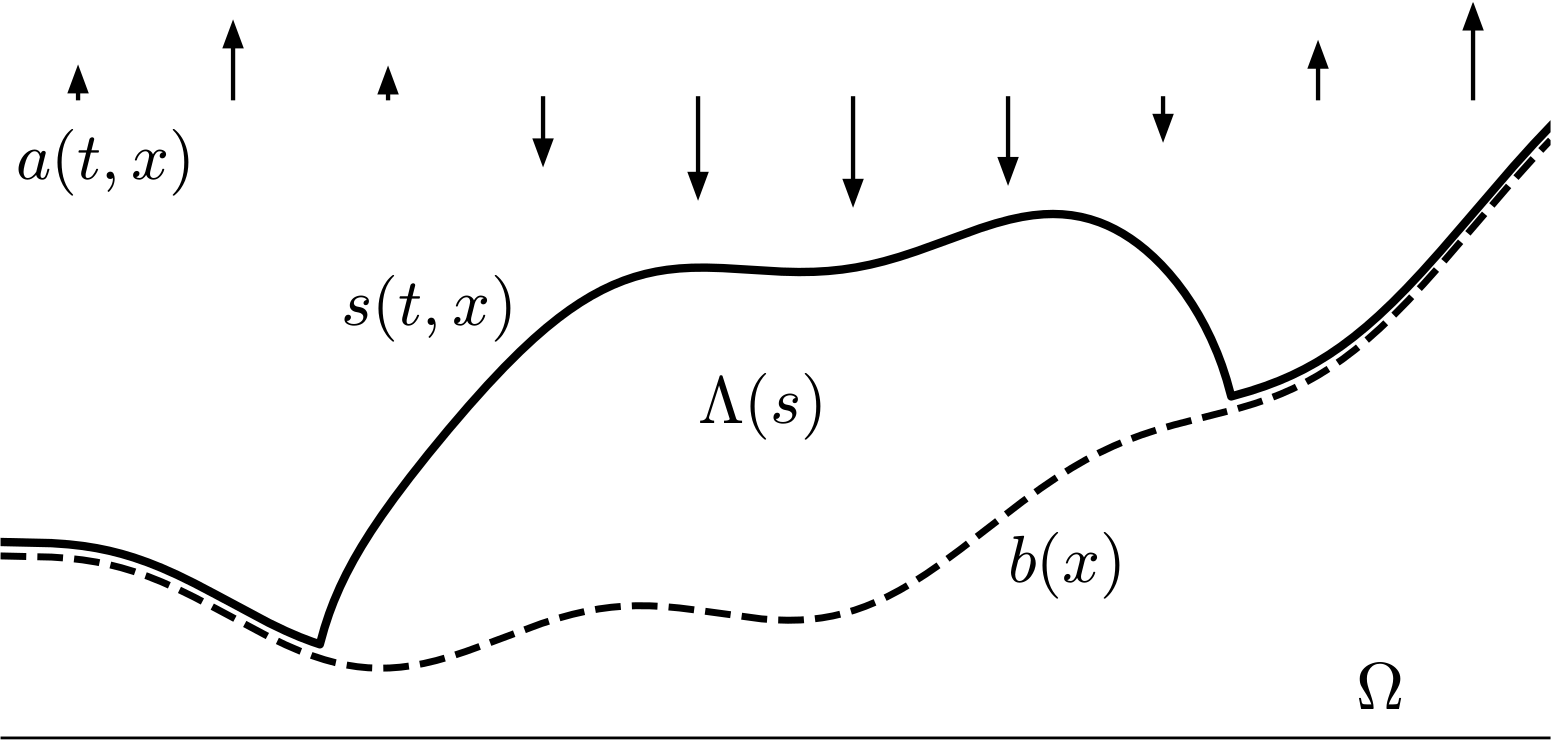
\includegraphics[width=0.65\textwidth]{genfigs/stokesdomain.pdf}
\caption{Glacier notation used in this paper.  In fact $\Omega$ is 2D and $\Lambda(t)$ is 3D.}
\label{fig:stokesdomain}
\end{figure}

Let $s(t,x)$ be the (solution) ice surface elevation.  We will regard this as defined for all $x\in\Omega$, and subject to the constraint that the surface $z=s$ must be at or above the bedrock ($s \ge b$).  In regions with no ice $s=b$ holds.  The solution ice velocity $\bu(t,x,z)$ and pressure $p(t,x,z)$ are then defined only on the open 3D domain
\begin{equation}
\Lambda(t) = \left\{(x,z)\,:\,b(x) < z < s(t,x)\right\} \subset \Omega \times \RR. \label{eq:icydomain}
\end{equation}
This aspect of glacier modeling deserves emphasis:  The time-dependent 3D domain $\Lambda(t)$, on which the solution velocity and pressure are meaningful, is determined by the evolving surface elevation $s(t,x)$, which is itself part of the model solution.

The surface trace of the ice velocity will be of importance, and it will be reconsidered in a precise Sobolev space context in Section \ref{sec:stokes}.  We extend it by zero so that it is defined everywhere in $\Omega$:
\begin{equation}
\bu|_s(t,x) = \begin{cases} \bu(t,x,s(t,x)), & s(t,x)>b(t,x) \\
                            \bzero, & \text{otherwise} .\end{cases} \label{eq:defineus}
\end{equation}
Compare flux extension by zero in \cite{SchoofHewitt2013}.

Let $\bn_s = \left<-\grad s,1\right>$ be an un-normalized and upward surface normal vector.  This is assumed well-defined for current purposes, but compare Section \ref{sec:model}.  Then an infinite-dimensional nonlinear complementarity problem (NCP) \cite{Bueler2021conservation,FacchineiPang2003,SchoofHewitt2013} applies almost everywhere in $[0,T]\times \Omega$:
\begin{subequations}
\label{eq:ncp}
\begin{align}
s - b &\ge 0 \\
\frac{\partial s}{\partial t} - \bu|_s \cdot \bn_s - a &\ge 0 \\
(s - b) \left(\frac{\partial s}{\partial t} - \bu|_s \cdot \bn_s - a\right) &= 0
\end{align}
\end{subequations}

System \eqref{eq:ncp} says that either a location is ice free ($s-b=0$), where the climate is locally ablating ($a\le 0$), or that the surface kinematical equation (SKE) holds:
\begin{equation}
\frac{\partial s}{\partial t} - \bu|_s \cdot \bn_s - a = 0.  \label{eq:ske}
\end{equation}
SKE \eqref{eq:ske} says that the (non-material) surface of the ice moves vertically according to the sum of the SMB and a component of the ice velocity at the surface \cite{SchoofHewitt2013}.  Equation \eqref{eq:ske} is a statement of mass conservation at the surface \cite{Aschwandenetal2012}, sometimes called the free-surface equation \cite{LofgrenAhlkronaHelanow2022} or the kinematic boundary condition\footnote{Note that equation \eqref{eq:ske} is not a boundary condition of any identifiable PDE problem.} \cite{GreveBlatter2009}.

We believe that glaciologists agree with the conditions of NCP \eqref{eq:ncp} as a model for glaciers.  For example, in numerical ice sheet models the SKE \eqref{eq:ske} is a standard way for surface geometry to evolve \cite{GreveBlatter2009,SchoofHewitt2013}.  The idea that positive (continuous) SMB at a given location implies the existence of glacier ice there is not controversial.  Equivalently, ice-free conditions are understood to exist only where the SMB is negative, because any accumulation (positive SMB) immediately becomes glacier ice by definition.

In the current paper the SMB $a$ is necessarily assumed to be defined everywhere in $\Omega$, regardless of whether a glacier is present or not.  At an ice-free location the SMB value can be modeled using precipitation and an energy balance \cite{GreveBlatter2009}, for instance by hypothesizing an ice or snow surface and then computing the balance of snow accumulation minus the total ablation from the energy available for melt.  Because a simulated glacier needs to be able to advance into unglaciated locations, the SMB there should have the value which a glacier surface would experience at that time and location.

The non-shallow ice dynamics model considered in this paper, which conserves mass and momentum, is a non-sliding (e.g.~frozen) base, isothermal, shear-thinning (non-Newtonian), and incompressible Stokes problem \cite{GreveBlatter2009,JouvetRappaz2011,SchoofHewitt2013}, applied over the domain $\Lambda(t)$ defined in \eqref{eq:icydomain}.  Let $\Gamma_s(t) \subset \partial \Lambda(t)$ be the upper surface $z=s$ and $\Gamma_b(t) \subset \partial \Lambda(t)$ be the base $z=b$.  The possibility of cliffs at the ice margin is neglected, so $\partial \Lambda(t) = \overline{\Gamma_s(t)} \cup \overline{\Gamma_b(t)}$ is assumed to hold at any time.  To state the shear-thinning (Glen's) flow law, let $D\bu=(\grad \bu + \grad \bu^{\top})/2$ denote the strain rate tensor, with Frobenius norm $|D\bu| = (D\bu:D\bu)^{1/2} = \left((D\bu)_{ij} (D\bu)_{ij}\right)^{1/2}$.  The effective ice (dynamic) viscosity \cite{GreveBlatter2009} is given by a regularized formula
\begin{equation}
\nu(D\bu) = \nu_\pp \left(\tfrac{1}{2} |D\bu|^2 + \eps\right)^{(\pp-2)/2} \label{eq:glen}
\end{equation}
The exponent $1 < \pp \le 2$, often written $\pp=(1/\nn)+1$, is approximately 4/3 in practice because $\nn\approx 3$ \cite{GreveBlatter2009}.  The coefficient $\nu_\pp>0$ has $\pp$-dependent units, but $\nu(D\bu)$ has SI units $\text{kg}\,\text{m}^{-1}\,\text{s}^{-1}$.  The values of $\nn$ and $\nu_\pp$ can be determined from measured properties of ice \cite{GoldsbyKohlstedt2001,GreveBlatter2009}, including temperature, but both are assumed to be constant (isothermal) here.  Note that $\pp=2$ yields a Newtonian fluid with constant viscosity, while for $\pp < 2$ the $\eps>0$ regularization implies that $\nu(D\bu)$ is bounded above.  Assume that the density of ice $\rhoi$ and the acceleration of gravity $\bg$ are constant.  At each time $t$ the modeled glacier has velocity and pressure solving the following 3D fluid equations:
\begin{subequations}
\label{eq:stokes}
\begin{align}
- \nabla \cdot \left(2 \nu(D\bu)\, D\bu\right) + \nabla p &= \rhoi \bg && \text{within $\Lambda(t)$} \\
\nabla \cdot \bu &= 0 && \qquad \text{''} \label{eq:stokes:incomp} \\
\left(2 \nu(D\bu) D\bu - pI\right) \bn_s &= \bzero && \text{on $\Gamma_s(t)$}\label{eq:stokes:stressfreesurface} \\
\bu  &= \bzero && \text{on $\Gamma_b(t)$} \label{eq:stokes:noslide}
\end{align}
\end{subequations}
Note that boundary condition \eqref{eq:stokes:stressfreesurface} says that the sub-aerial upper surface is stress free; this must not be confused with the SKE \eqref{eq:ske}.

In summary at this point, we assume that a glacier simulation is an evolving free-surface flow, subject to a signed climate that can add or remove ice, coupled to a nonlinear Stokes problem which must be solved within an evolving, 3D icy domain.  The initial/boundary value problem consisting of \eqref{eq:icydomain}--\eqref{eq:stokes} requires data $b(x),a(t,x)$ plus an initial surface elevation $s(0,x)$.  The solution variables are $s(t,x)$, $\bu(t,x,z)$, and $p(t,x,z)$, with $s$ defined everywhere over $[0,T]\times \Omega$, but subject to $s \ge b$, and with $\bu,p$ defined on $\Lambda(t)$ for each $t$.  The surface elevation $s$ and surface velocity $\bu|_s$ are linked by the kinematical NCP \eqref{eq:ncp}.

Note that the NCP \eqref{eq:ncp} is the only place where a time derivative appears in the model statement; the SKE \eqref{eq:ske} is implied by the NCP.  Because the flow is very viscous \cite{Acheson1990}, the Stokes sub-model \eqref{eq:glen}--\eqref{eq:stokes} acts as an instantaneous ``algebraic'' constraint on the evolution statement in \eqref{eq:ncp}.  The coupled, infinite-dimensional problem of determining the evolving geometry of a glacier, namely system \eqref{eq:icydomain}--\eqref{eq:stokes}, is therefore simultaneously a differential algebraic equation system \cite{AscherPetzold1998,LofgrenAhlkronaHelanow2022} and an NCP.

While essentially equivalent in the continuum problem, formulations using thickness functions to parameterize geometry have different character from those using surface elevation, as here, when the bedrock is realistically rough.  Surface elevation $s$ will be preferred because of the flow-caused smoothing effect illustrated in Figure \ref{fig:giscross}.  That is, we observe that for land-based glaciers $s(t,x)$ is smoother in $x$ than the thickness $H(t,x) = s(t,x)-b(x)$ because the latter ``inherits'' the lower regularity of the (typically) eroded and/or faulted bedrock topography $b(x)$.

\begin{figure}
\begin{minipage}[t]{0.85\textwidth}
\vspace{0pt}
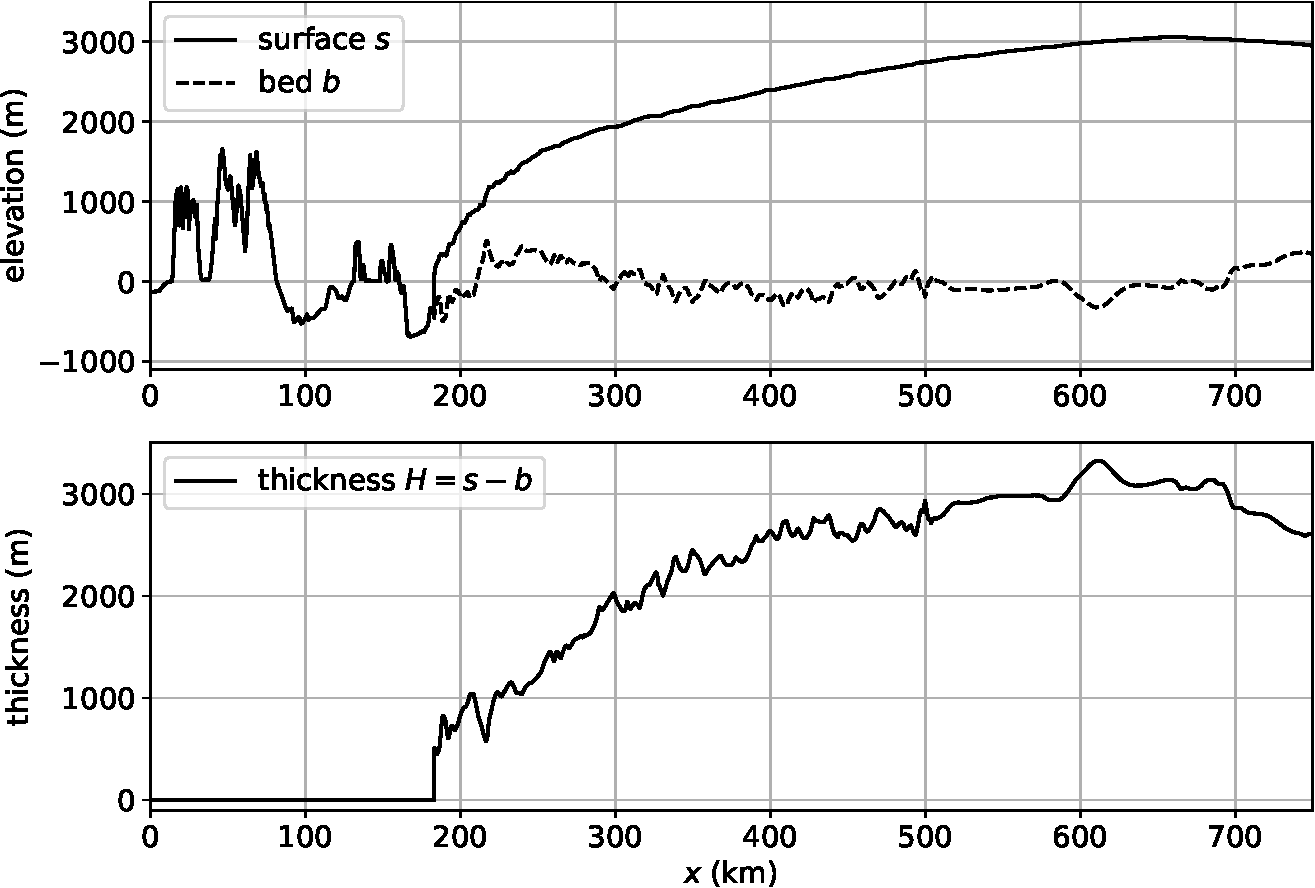
\includegraphics[width=\textwidth]{genfigs/giscross.pdf}
\end{minipage}
\,
\begin{minipage}[t]{0.13\textwidth}
\vspace{10pt}
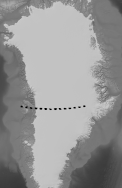
\includegraphics[width=\textwidth]{genfigs/gis/gris-profile-gray.png}
\end{minipage}
\caption{A cross-section of the Greenland ice sheet at $70^\circ$N latitude (see inset).  While the ice surface $s$ is relatively smooth because of ice flow (top), the bedrock elevation $b$ is much rougher.  The corresponding ice thickness $H = s-b$ (bottom), though a valid geometry parameterization, inherits the low regularity of $b$.  (Data from \cite{Morlighemetal2017} and A.~Aschwanden, personal communication.)}
\label{fig:giscross}
\end{figure}

Glacier simulations are commonly formulated using a finite element (FE) method for the Stokes sub-problem \cite{IsaacStadlerGhattas2015,Jouvetetal2008,Pattynetal2008}, or for a shallow approximation thereof.  However, to the author's knowledge all existing non-shallow (Stokes) evolution models use a explicit time-stepping scheme for the geometry, for example as in \cite{Jouvetetal2008} or \cite{LofgrenAhlkronaHelanow2022}, with the one exception of the exploratory model in reference \cite{WirbelJarosch2020}.

This work instead considers implicit time steps for the theoretical reasons addressed in Section \ref{sec:theory}.  For a time step $\Delta t > 0$, the solution $s\approx s(t_n,x)$, from applying the backward Euler scheme to NCP \eqref{eq:ncp} satisfies the conditions of a similar NCP:
\begin{subequations}
\label{eq:be:ncp}
\begin{align}
s - b &\ge 0 \label{eq:be:ncp:constraint} \\
s - \Delta t\,\bu|_s \cdot \bn_s - \ell^n &\ge 0 \label{eq:be:ncp:residualpos} \\
(s - b) \left(s - \Delta t\,\bu|_s \cdot \bn_s - \ell^n\right) &= 0 \label{eq:be:ncp:complementarity}
\end{align}
\end{subequations}
For clarity we have collected-together a source term $\ell^n(x) = s^{n-1}(x) + \int_{t_{n-1}}^{t_n} a(t,x)\,dt$, which is assumed known.

Observe that the backward Euler scheme chosen for problem \eqref{eq:be:ncp} is merely the simplest A-stable \cite{AscherPetzold1998} scheme which can be applied to the continuous time problem \eqref{eq:ncp}.  For finite-dimensional differential algebraic equation problems, such implicit and A-stable schemes are the standard choices \cite{AscherPetzold1998}, given the stiffness exhibited by such systems.  Applying the same strategy in the infinite-dimensional case here, i.e.~where the SKE \eqref{eq:ske} is constrained at any time by the ``algebraic'' Stokes problem \eqref{eq:glen}--\eqref{eq:stokes}, is therefore natural.

One can also make a case for implicit time-stepping based on simulation performance, that is, compared to the conditionally-stable explicit alternative \cite{Bueler2023}.  This assumes that NCP \eqref{eq:be:ncp} can be solved efficiently, and that the implicit scheme turns out to have unconditional stability.  However, neither efficiency nor stability are addressed in the current paper.

The essential approach of this paper starts in Section \ref{sec:model}, where we re-write NCP \eqref{eq:be:ncp} as a weak form VI problem.  Based on conjectured well-posedness for that problem (Section \ref{sec:theory}), our main results are in Sections \ref{sec:abstractestimate} and \ref{sec:application}.  We prove new estimates on the numerical error which arises from solving the VI problem by finite element (FE) approximation.

In fact this paper is organized as follows.  Section \ref{sec:stokes} recalls the theory of the Glen-law Stokes problem on a fixed domain, but we add an apparently-new bound on the surface trace of the velocity solution (Corollary \ref{cor:surfacetracebound}).  In Section \ref{sec:model} we reformulate the coupled NCP problem \eqref{eq:glen}--\eqref{eq:be:ncp} as a VI weak form.  The key coupling term is the surface motion term $\bu|_s\cdot \bn_s$ in SKE \eqref{eq:ske}, for which we provide a quantitative bound over a Sobolev space of surface elevation functions (Lemma \ref{lem:philipschitz}).  However, this bound is subject to Conjecture \ref{conj:a}, which hypothesizes that the surface velocity trace is Lipschitz continuous with respect to surface elevation.  Well-posedness for each implicit step VI problem is considered in Section \ref{sec:theory}, based upon Conjecture \ref{conj:b} hypothesizing the coercivity of the same surface motion term.  Certain physical and modeling ideas are discussed in Section \ref{sec:theory}, as context needed to understand Conjecture \ref{conj:b}, followed by some numerical evidence for the validity of the Conjecture \ref{conj:b} in Section \ref{sec:numerical}, via Stokes glacier simulations in 2D.  At this point we have in hand a mathematically-precise time-discretized model, though with only conjectural well-posedness; see Theorem \ref{thm:stepwellposed}.  This continuum model, apparently stated here for the first time, can be approximated by an FE method.  In Section \ref{sec:abstractestimate} we prove an abstract FE error estimate, Theorem \ref{thm:abstractestimate} and its Corollaries, for general VI problems involving nonlinear operators on Banach spaces.  This new estimate, which makes coercivity and Lipshitz assumptions on the operator, extends the classical bilinear case by Falk \cite{Falk1974}.  In Section \ref{sec:application} we apply the abstract estimate to the glacier model, yielding our final result which is Theorem \ref{thm:glacierapp}.  The physical significance of each term in this error estimate, and how associated FE method choices are made, is addressed at the end.

We will use only a few mathematical and glaciological abbreviations: FE (finite element), NCP (nonlinear complementarity problem), PDE (partial differential equation), SIA (shallow ice approximation), SKE (surface kinematical equation), SMB (surface mass balance), and VI (variational inequality).


\section{The surface velocity from a glacier Stokes problem} \label{sec:stokes}

In this Section we consider the weak form of the non-sliding, isothermal, and Glen-law Stokes sub-model \eqref{eq:glen}--\eqref{eq:stokes}.  This sub-model, which is applied on a fixed 3D domain $\Lambda = \Lambda(t)$, defined by \eqref{eq:icydomain} at a particular time $t$, computes the surface velocity field $\bu|_s$ which appears in NCP \eqref{eq:ncp}.  (We return to that the larger model in Section \ref{sec:model}.)  We assume in the current Section that the ice base $\Gamma_b\subset\partial \Lambda$, on which a Dirichlet condition $\bu=\bzero$ holds, has positive measure, and that the remaining Neumann boundary $\Gamma_s = \partial \Lambda \setminus \overline{\Gamma_b}$ is sufficiently-smooth so that a zero normal stress condition can be applied.

Suitable function spaces for Stokes problem \eqref{eq:glen}--\eqref{eq:stokes} are well-known so long as the domain $\Lambda$ is sufficiently regular.  Let $1 < \pp \le 2$, and recall that $\pp=(1/\nn)+1\approx 4/3$ in viscosity formula \eqref{eq:glen}.  Denote the Sobolev space \cite{Evans2010} of real-valued functions with $\pp$th-power integrable first derivatives by $W^{1,\pp}(\Lambda)$.  Let
\begin{equation}
\cV = W_b^{1,\pp}(\Lambda; \RR^3) \label{eq:defineV}
\end{equation}
be the corresponding space of vector-valued functions with value (trace) zero along $\Gamma_b$.  Let $[H]>0$ be a representative \emph{vertical} glacier dimension.  We define the norm on $\cV$ by
\begin{equation}
\|\bv\|_{\cV} = \left(\int_\Lambda |\bv|^\pp\,dx\,dz + [H]^\pp \int_\Lambda |\grad\bv|^\pp\,dx\,dz\right)^{1/\pp}. \label{eq:vnorm}
\end{equation}
Here $dx\,dz = dx_1\,dx_2\,dz$ is the 3D volume element, which will generally be suppressed from now on in integrals.  Note that $|\bv|$ denotes the Euclidean norm of $\bv\in\RR^3$ and $|\grad\bv|=\left((\grad\bv)_{ij} (\grad\bv)_{ij}\right)^{1/2}$ is the Frobenius norm of $\grad\bv\in\RR^{3\times 3}$.  Remark 1.2.1 in \cite{BoffiBrezziFortin2013} explains the length scaling in \eqref{eq:vnorm}, such that $\|\bv\|_{\cV}$ has consistent units.  We will assume throughout that $[H] \ge 1$ m.

Let $\cQ=L^{\pp'}(\Lambda)$ where $\pp'=\pp/(\pp-1)\approx 4$ is the conjugate exponent.  Define
\begin{equation}
\mathcal{M} = \cV \times \cQ \label{eq:glenstokes:mixedspace}
\end{equation}
as the mixed space of admissible velocity and pressure pairs.  For $(\bu,p) \in \mathcal{M}$ define
\begin{equation}
F_\Lambda(\bu,p)[\bv,q] = \int_\Lambda 2 \nu(D\bu) D\bu : D\bv - p \Div\bv - (\Div\bu) q - \rhoi \bg \cdot \bv. \label{eq:glenstokes:fcnl}
\end{equation}
The (mixed) weak form of the Stokes sub-model seeks the solution $(\bu,p)$ satisfying
\begin{equation}
F_\Lambda(\bu,p)[\bv,q] = 0 \qquad \text{for all } (\bv,q) \in \mathcal{M}. \label{eq:glenstokes:weak}
\end{equation}

Jouvet and Rappaz \cite{JouvetRappaz2011} have proven that problem \eqref{eq:glenstokes:weak} is well-posed if the Neumann portion of $\partial\Lambda$ is $C^1$.  Their proof uses the equivalence of \eqref{eq:glenstokes:weak} and the minimization of a convex and coercive functional over the divergence-free subspace $\Vdiv = \{\bv\in\cV\,:\,\Div\bv=0\}$.  Our regularization in Glen law \eqref{eq:glen} differs from that in \cite{JouvetRappaz2011}, but the necessary modifications are addressed in \cite{IsaacStadlerGhattas2015}.  Note that if the weak solution is sufficiently regular then the strong form \eqref{eq:stokes} is also satisfied.

\begin{theorem}[Theorem 3.10 in \cite{JouvetRappaz2011} and Appendix A of \cite{IsaacStadlerGhattas2015}] \label{thm:stokeswellposed}  Suppose $\Lambda$ is bounded, $\partial\Lambda$ is Lipschitz, $\Gamma_s$ is $C^1$, and $\Gamma_b$ has positive measure.  Let $1<\pp\le 2$ and $\eps>0$ in \eqref{eq:glen}.  Then there exists a unique pair $(\bu,p) \in \mathcal{M}$ solving \eqref{eq:glenstokes:weak}, and $\bu\in \Vdiv$.
\end{theorem}

Our primary purpose, resumed in the next Section, is to study the glacier geometry NCP \eqref{eq:ncp}, and its weak form.  For that analysis we need to bound the surface trace $\bu|_s$ in terms of certain geometric properties of $\Lambda$.  This uses several inequalities.

\begin{lemma}[Poincar\'e's inequality; (7.44) in \cite{GilbargTrudinger2001}] \label{lem:poincare}
Under the assumptions of Theorem \ref{thm:stokeswellposed}, there exists a dimensionless constant $c_{\pp}(\Lambda)>0$ so that
\begin{equation}
\int_\Lambda |\bv|^\pp \le c_{\pp}(\Lambda) [H]^\pp \int_\Lambda |\grad\bv|^\pp \qquad \text{for all } \bv \in \cV. \label{eq:poincare}
\end{equation}
\end{lemma}

Lemma \ref{lem:poincare} shows that $\|\bv\|_{\cV}^\pp \le (c_{\pp}(\Lambda) + 1) [H]^\pp \int_\Lambda |\grad\bv|^\pp$ for $\bv \in \cV$.
 
\begin{lemma}[Korn's inequality; to prove this set $F(x)$ to the identity in Corollary 4.1 of \cite{Pompe2003}] \label{lem:korns}
Under the same assumptions, there exists a dimensionless constant $k_{\pp}(\Lambda)>0$ so that
\begin{equation}
\int_\Lambda |\grad\bv|^\pp \le k_{\pp}(\Lambda) \int_\Lambda |D\bv|^\pp \qquad \text{for all } \bv \in \cV. \label{eq:korns}
\end{equation}
\end{lemma}

The main idea of the following \emph{a priori}  bound is that velocity is controlled by geometric properties of the domain $\Lambda$, including the constants in the above inequalities, along with certain physical constants.  We will denote the ice volume by $|\Lambda|$.

\begin{lemma} \label{lem:stokesapriori}
Suppose $\bu\in\cV$ is the Stokes velocity solution from Theorem \ref{thm:stokeswellposed}.  Then there is $C>0$ depending on $\pp$, $\rhoi |\bg|$, $\nu_\pp$, $\eps$, $[H]$, $|\Lambda|$, $c_\pp(\Lambda)$, and $k_\pp(\Lambda)$, but not on $\bu$, so that
\begin{equation}
\|\bu\|_{\cV} \le C. \label{eq:stokesapriori}
\end{equation}
\end{lemma}

\begin{proof}
From \eqref{eq:glenstokes:weak} and $\bu \in\Vdiv$ it follows that
\begin{equation}
0= F_\Lambda(\bu,p)[\bu,p] = \int_\Lambda 2 \nu(D\bu) D\bu : D\bu - \rhoi \bg \cdot \bu.  \label{eq:stokes:substituteu}
\end{equation}
Apply Korn's inequality, the facts that $\pp>0$ and $(\pp-2)/2 \le 0$, and equation \eqref{eq:glen}:
\begin{align}
\int_\Lambda |\grad\bu|^\pp &\le k_{\pp}(\Lambda) \int_\Lambda |D\bu|^\pp \le k_{\pp}(\Lambda) \int_\Lambda \left(|D\bu|^2 + \eps\right)^{(\pp-2)/2} \left(D\bu:D\bu + \eps\right) \label{eq:stokes:startapriori} \\
	&= k_{\pp}(\Lambda) \left[\eps^{\pp/2} |\Lambda| + (2 \nu_\pp)^{-1} \int_\Lambda \nu(D\bu) D\bu:D\bu\right]. \notag
\end{align}
By equation \eqref{eq:stokes:substituteu} and H\"older's inequality we thus have
\begin{align}
\int_\Lambda |\grad\bu|^\pp &\le k_{\pp}(\Lambda) \left[\eps^{\pp/2} |\Lambda| + (2 \nu_\pp)^{-1} \int_\Lambda \rhoi \bg \cdot \bu\right] \label{eq:stokes:workapriori} \\
	&\le k_{\pp}(\Lambda) \left[\eps^{\pp/2} |\Lambda| + (2 \nu_\pp)^{-1} \rhoi |\bg| |\Lambda|^{1/\pp'} \|\bu\|_\cV\right]. \notag
\end{align}
(This assumes that $\rhoi$ and $|\bg|$ are constant.)  By the comment after Lemma \ref{lem:poincare},
\begin{equation}
\|\bu\|_{\cV}^\pp \le (c_{\pp}(\Lambda) + 1) [H]^\pp k_{\pp}(\Lambda) \left[\eps^{\pp/2} |\Lambda| + (2 \nu_\pp)^{-1} \rhoi |\bg| |\Lambda|^{1/\pp'} \|\bu\|_\cV\right].
\end{equation}

Let $z=\|\bu\|_\cV$.  We have proved that
\begin{equation}
z^\pp \le c_0 + c_1 z
\end{equation}
for $\pp>1$ and some constants $c_i>0$.  Note that $g(y) = y^\pp - c_1 y - c_0$ is smooth with $g(0)=-c_0<0$ and $g(y) \to +\infty$ as $y \to +\infty$, so there exists a right-most root $\tilde y>0$ with $\tilde y = f(\pp,c_0,c_1)$.  Since $g(z)\le 0$ we have $z \le \tilde y$.  This proves \eqref{eq:stokesapriori} with $C=\tilde y$.
\end{proof}

\begin{lemma}[Trace inequality] \label{lem:trace}
Under the assumptions of Theorem \ref{thm:stokeswellposed}, there exists a dimensionless constant $\gamma_{\pp}(\Lambda)>0$ so that for all $\bv \in \cV$,
\begin{equation}
\int_{\Gamma_s} |\bv|^\pp \,dS \le \frac{\gamma_{\pp}(\Lambda)}{[H]} \|\bv\|_{\cV}^\pp \label{eq:trace}
\end{equation}
where $\bv$ on the left is the trace on $\Gamma_s$, and $dS$ denotes the area element over $\partial\Lambda$.
\end{lemma}

\begin{proof}
Theorem 5.5.1 in \cite{Evans2010} defines a trace operator $T:\cV\to L^\pp(\partial\Lambda)$, and a constant $c>0$, dependent only on $\pp$ and $\Lambda$, so that
\begin{equation}
\int_{\partial\Lambda} |T\bv|^p\,dS \le c \int_{\Lambda} |\bv|^\pp + |\grad\bv|^\pp \label{eq:tracework}
\end{equation}
for $\bv\in\cV$.  However, because $\bv=\bzero$ along $\Gamma_b$, clearly $\int_{\Gamma_s} |T\bv|^\pp\,dS = \int_{\partial\Lambda} |T\bv|^\pp\,dS$.  The result follows if we define $\gamma_{\pp}(\Lambda)=[H] c$.
\end{proof}

Combining Lemmata \ref{lem:stokesapriori} and \ref{lem:trace} yields the following bound.  In using this result, recall that $\Lambda$ is determined by $s$ and $b$, i.e.~as in definition \eqref{eq:icydomain}.

\begin{corollary}[Surface velocity bound] \label{cor:surfacetracebound}
Suppose $\bu\in\cV$ is the Stokes velocity solution from Theorem \ref{thm:stokeswellposed}.  The norm of its trace over $\Gamma_s$ is controlled, \emph{a priori}, by $[H]$, $C$ in \eqref{eq:stokesapriori}, and $\gamma_{\pp}(\Lambda)$ in \eqref{eq:trace}:
\begin{equation}
\int_{\Gamma_s} |\bu|^\pp \,dS \le \frac{\gamma_{\pp}(\Lambda)}{[H]} C^\pp. \label{eq:surfacetracebound}
\end{equation}
\end{corollary}


\section{The weak-form implicit time-step model} \label{sec:model}

Now we return to the implicit time-stepping scheme for updating the surface elevation in a model based on Stokes dynamics, namely NCP \eqref{eq:be:ncp}.  Recall how this problem is derived.  Let $\{t_n\}$ be any increasing sequence of times in $[0,T]$, with $t_0=0$.  Let $\Delta t = t_n-t_{n-1}$ denote the generic step length.  Let $a^n(x)$ be the (temporal) average of the data $a(t,x)$ over $[t_{n-1},t_n]$.  Suppose that $s(x)=s^n(x)\approx s(t_n,x)$ approximates the surface elevation at time $t_n$.  Using a backward Euler implicit step \cite{AscherPetzold1998}, SKE \eqref{eq:ske} becomes
\begin{equation}
\frac{s - s^{n-1}}{\Delta t} - \bu|_{s} \cdot \bn_{s} - a^n = 0. \label{eq:be:ske}
\end{equation}
(Importantly, the unknown $s=s^n$ appears both in the surface velocity $\bu|_s$ and slope $\bn_s$.)  For cleaner appearance, clear the denominator in \eqref{eq:be:ske} and define
\begin{equation}
\ell^n(x) = s^{n-1}(x)+\Delta t\,a^n(x) = s^{n-1}(x) + \int_{t_{n-1}}^{t_n} a(t,x)\,dt. \label{eq:be:source}
\end{equation}
As noted in the Introduction, $s=s^n$ in \eqref{eq:be:ske} actually solves a problem of free-boundary type, which is NCP \eqref{eq:be:ncp}.  In particular, complementarity equation \eqref{eq:be:ncp:complementarity} says that, at the solution time and almost everywhere over $\Omega$, either there is no ice ($s=b$) or equation \eqref{eq:be:ske} holds.  Notice that $s$ does not solve \eqref{eq:be:ske} over the bare ground part of $\Omega \subset \RR^2$ where $s=b$.

The strong form NCP \eqref{eq:be:ncp} has a weak-form variational inequality (VI; \cite{Evans2010,KinderlehrerStampacchia1980}) version which is better-suited to both well-posedness theory and finite element (FE) analysis.  Let us regard the precise Banach space $\cX$ of surface elevations as unknown.  The admissible surface elevations come from a convex and closed subset
\begin{equation}
\cK = \left\{r \in\cX\,:\,r|_{\partial\Omega}=b|_{\partial\Omega} \text{ and } r \ge b\right\}.  \label{eq:be:admissible}
\end{equation}
While the fixed (Dirichlet) boundary condition is included into the definition of $\cK$, if the glacier does not reach $\partial\Omega$ then this condition is of little importance.  The VI is then derived as follows via the argument from \cite{Bueler2021conservation}.  Suppose that $s \in \cK$ is a sufficiently-regular solution of NCP \eqref{eq:be:ncp}.  Let $\Omega_I$ be the (measurable) subset of $\Omega$ on which constraint \eqref{eq:be:ncp:constraint} is inactive, where glacier ice is present: $\Omega_I = \{x\,:\,s(x)>b(x)\}$.  From \eqref{eq:be:ncp:complementarity}, integration over $\Omega_I$ shows that
\begin{equation}
\int_{\Omega_I} \left(s - \Delta t\,\bu|_s \cdot \bn_s - \ell^n\right)\,(r-s) = 0  \label{eq:inactivetruth}
\end{equation}
for any $r\in\cK$.  On the other hand, suppose $\Omega_A = \{x \in \Omega \,:\,s(x)=b(x)\}$ is the active (ice-free) region for constraint \eqref{eq:be:ncp:constraint}.  Observe that \eqref{eq:be:ncp:residualpos} says that $b-\ell^n = s - \Delta t\,\bu|_s \cdot \bn_s - \ell^n \ge 0$ on $\Omega_A$.\footnote{Otherwise, physically speaking, and assuming continuity of $b$, $s^{n-1}$, and $a^n$, a glacier would still be present somewhere in $\Omega_A$, or would have appeared during the time step, a contradiction.  Note the role of extension by zero \eqref{eq:defineus} here.}  Note that $r-s=r-b\ge 0$ on $\Omega_A$ if $r\in\cK$.  Therefore, because $b-\ell^n \ge 0$ and $r-s\ge 0$ on $\Omega_A$, integration yields an inequality:
\begin{equation}
\int_{\Omega_A} \left(s - \Delta t\,\bu|_s \cdot \bn_s - \ell^n\right)\,(r-s) = \int_{\Omega_A} \left(b - \ell^n\right)\,(r-b) \ge 0.  \label{eq:activetruth}
\end{equation}
Either land is glacier covered (within $\Omega_I$) or ice-free ($\Omega_A$), so addition of \eqref{eq:inactivetruth} and \eqref{eq:activetruth} gives the following VI for $s \in \cK$:
\begin{equation}
\int_\Omega \left(s - \Delta t\,\bu|_s \cdot \bn_s\right)\,(r-s) \ge \int_\Omega \ell^n \,(r-s) \quad \text{for all } r \in \cK. \label{eq:be:viearly}
\end{equation}
This integral inequality is known to be true of $s\in\cK$ in advance of knowledge about the ice-covered part of $\Omega$.
	
Now, well-posedness of the weak-form Stokes problem \eqref{eq:glenstokes:weak} over a 3D domain $\Lambda$, plus the surface trace bound in Corollary \ref{cor:surfacetracebound}, allows us to create a well-defined map from an admissible surface elevation $s$ to the corresponding surface velocity solution $\bu|_s$.  The map is defined via definition \eqref{eq:icydomain}, followed by the solution of \eqref{eq:glenstokes:weak} over $\Lambda$, evaluation of the trace of $\bu$ along $\Gamma_s$ (Corollary \ref{cor:surfacetracebound}), and then definition \eqref{eq:defineus} (which includes extension by zero).  For this map to be well-defined, $s$ must admissible ($s\in\cK$) and it must be sufficiently regular so that these steps are justified.  In fact, we call
\begin{equation}
\Phi(s) = - \bu|_s\cdot \bn_s \label{eq:definePhi:asfunction}
\end{equation}
the \emph{surface motion map}.  It maps the scalar surface elevation $s$ to the scalar dynamical term in the SKE \eqref{eq:be:ske}.  Constructing a bound for $\Phi$ will help to identify a Banach space $\cX$ in which to seek admissible solutions $s$.

As before, let $\Omega \subset \RR^2$ be a bounded domain and let $[L]>0$ be a representative \emph{horizontal} scale; compare \eqref{eq:vnorm}.  For any $\rr\ge 1$ and $q\in W^{1,\rr}(\Omega)$ we define
\begin{equation}
\|q\|_{W^{1,\rr}} = \left(\int_\Omega |q|^\rr\,dx + [L]^\rr \int_\Omega |\grad q|^\rr\,dx\right)^{1/\rr}. \label{eq:norm:Omega}
\end{equation}

\begin{lemma}[Preliminary bound on $\Phi(s)$] \label{lem:phibound:early}  Suppose $2 \le \rr \le \infty$, and assume $s\in W^{1,\rr}(\Omega)$ is admissible ($s\ge b$).  With $\Lambda$ defined by \eqref{eq:icydomain}, assume that the hypotheses of Theorem \ref{thm:stokeswellposed} and Corollary \ref{cor:surfacetracebound} apply, which also shows that $\Phi(s)$ is a well-defined measurable function.  Then there is a constant $C>0$ independent of $\qq$ so that
\begin{equation}
\left|\int_\Omega \Phi(s) q\,dx\right| = \left|\int_\Omega \bu|_s\cdot \bn_s q\,dx\right| \le C\, \|q\|_{W^{1,\rr}} \qquad \text{for all } q\in W^{1,\rr}(\Omega).  \label{eq:phibound:early}
\end{equation}
\end{lemma}

\begin{proof}  Observe that $dS = |\bn_s|\,dx = \sqrt{1+|\grad s|^2}\,dx$ is the surface area element for $\Gamma_s \subset \partial \Lambda$.  Recall from Section \ref{sec:stokes} that $\pp=1+1/\nn \approx 4/3$.  Let $\pp'=\pp/(\pp-1) \approx 4$ be the conjugate exponent.  Apply the triangle inequality, and H\"older's inequality twice:
\begin{align}
\left|\int_\Omega \Phi(s) q\,dx\right| &\le \int_\Omega \big|\bu|_s\big| |\bn_s| |q|\,dx = \int_\Omega \big|\bu|_s\big| |\bn_s|^{1/\pp} |\bn_s|^{1/\pp'} |q|\,dx \label{eq:phibound:zero} \\
    &\le \left(\int_\Omega \big|\bu|_s\big|^\pp |\bn_s|\,dx\right)^{1/\pp} \left(\int_\Omega |\bn_s| |q|^{\pp'} \,dx\right)^{1/\pp'} \notag \\
    &\le \left(\int_{\Gamma_s} |\bu|^\pp \,dS\right)^{1/\pp} \left(\int_\Omega |\bn_s|^\rr \,dx\right)^{1/(\pp'\rr)} \left(\int_\Omega |q|^{\pp'\rr'} \,dx\right)^{1/(\pp'\rr')}. \notag
\end{align}
If $C_1$ is the \emph{a priori} bound from \eqref{eq:surfacetracebound} then
\begin{equation}
\left|\int_\Omega \Phi(s) q\,dx\right| \le C_1^{1/\pp} \left(\int_\Omega \left(1+|\grad s|^2\right)^{\rr/2}\,dx\right)^{1/(\pp'\rr)} \|q\|_{L^{\pp'\rr'}}.
\end{equation}
Note that if $\alpha\ge 0$ then $(1+\alpha)^{\rr/2} \le 2^{(\rr-2)/2} (1+\alpha^{\rr/2})$, so
\begin{align}
\left|\int_\Omega \Phi(s) q\,dx\right| &\le C_1^{1/\pp} \left(2^{(\rr-2)/2} \int_\Omega 1 + |\grad s|^\rr\,dx\right)^{1/(\pp'\rr)} \|q\|_{L^{\pp'\rr'}} \label{eq:phibound:one} \\
  &\le C_2 \left(|\Omega| + [L]^{-\rr}\|s\|_{W^{1,\rr}}^\rr\right)^{1/(\pp'\rr)} \|q\|_{L^{\pp'\rr'}}. \notag
\end{align}
Since $2 \le \pp' \le \pp'\rr' < \infty$, by Sobolev's inequality\footnote{For example, apply Theorem 8.8 from \cite{LiebLoss1997} using $n=2$, $k=m=1$, $p=\rr$, and $q=\pp'\rr'$.} we also have $\|q\|_{L^{\pp'\rr'}} \le C_3 \|q\|_{W^{1,\rr}}$, which yields \eqref{eq:phibound:early}.
\end{proof}

The key assumption in Lemma \ref{lem:phibound:early} is that $s\in W^{1,\rr}(\Omega)$ implies that the domain $\Lambda$ is nice enough so that Corollary \ref{cor:surfacetracebound} gives a finite bound.  The key conclusion is that $\Phi(s) \in \left(W^{1,\rr}(\Omega)\right)'$, the dual space.  This conclusion will be critical in analyzing the weak form of NCP \eqref{eq:be:ncp}.

Now we conjecture that for some\footnote{The reason for requiring $\rr>2$ will be seen in Lemma \ref{lem:philipschitz}.  It would seem to be a technical requirement, as Section \ref{sec:application} demonstrates well-behaved numerical results using the more convenient exponent $\rr=2$.} $\rr>2$, the $L^{\rr'}$-norm of the surface trace $\bu|_s$ is Lipschitz as a function of $s \in W^{1,\rr}(\Omega)$.  Note that we do not assume that $\bu|_s$ is continuous, only that it is a measurable function defined over all of $\Omega$.

\begin{conjecture} \label{conj:a}  There exists $2 < \rr \le \infty$ with the following two properties:  \emph{(i)} If $s\in W^{1,\rr}(\Omega)$ is admissible ($s\ge b$ and $s=b$ on $\partial\Omega$) then the conclusion of Theorem \ref{thm:stokeswellposed} applies, giving a well-defined surface velocity $\bu|_s$.  \emph{(ii)} If also $r\in W^{1,\rr}(\Omega)$ is admissible, yielding different values $\bu|_r$, then there exists $\CA>0$, independent of $s$ and $r$, such that
\begin{equation}
\big\|\bu|_r - \bu|_s\big\|_{L^{\rr'}} \le \CA \|r-s\|_{W^{1,\rr}}. \label{eq:ulipschitz}
\end{equation}
\end{conjecture}

From now on we will assume Conjecture \ref{conj:a} holds for some $2 < \rr \le \infty$.  We define
\begin{equation}
\cX = W^{1,\rr}(\Omega). \label{eq:defineX}
\end{equation}
Since $\rr>2$ we have $\cX \hookrightarrow C(\bar\Omega)$.  Definition \eqref{eq:be:admissible} again describes the closed and convex admissible subset $\cK \subset \cX$.  If $s\in\cK$ then, by Conjecture \ref{conj:a}, $\bu|_s\cdot\bn_s$ is a measurable, real-valued function on $\Omega$.  For $q\in\cX$ we will, from now on, write $\Phi(s)$ as a linear functional:
\begin{equation}
\Phi(s)[q] = -\int_\Omega \bu|_s\cdot\bn_s\,q\,dx. \label{eq:definePhi}
\end{equation}
Lemma \ref{lem:phibound:early} has shown that $\Phi$ maps from $\cK$ to the (topological) dual space $\cX'$.  Note that $\Phi(s)[q]$ is nonlinear in $s$ but linear in $q$.  The next Lemma simply proves that $\Phi$ is also Lipschitz-continuous if we assume Conjecture \ref{conj:a}.

\begin{lemma} \label{lem:philipschitz}  Suppose that Conjecture \ref{conj:a} holds.  Fix $b \in \cX$ and use definition \eqref{eq:be:admissible} to define $\cK$.  The map $\Phi:\cK\to\cX'$ is Lipschitz on bounded subsets of $\cK$, that is, for each $R>0$ there is $C(R)>0$ so that if $r,s\in B_R \cap \cK = \{t\in \cK\,:\,\|t\|_{\cX} \le R\}$ and $q\in\cX$ then
\begin{equation}
\Big|\Phi(r)[q] - \Phi(s)[q]\Big| \le C(R)\, \|r-s\|_{\cX} \|q\|_{\cX}  \label{eq:philipschitz}
\end{equation}
\end{lemma}

\begin{proof}  Suppose $s,r\in\cK$.  Add and subtract $\bu|_s \cdot \bn_r$, and apply triangle inequalities, including $|\bn_r|=\left(1+|\grad r|^2\right)^{1/2} \le 1 + |\grad r|$:
\begin{align}
\big|\Phi(r)[q] - \Phi(s)[q]\big| &\le \int_\Omega \big|\bu|_r - \bu|_s\big| |\bn_r| |q|\,dx + \int_\Omega \big|\bu|_s\big| |\bn_r-\bn_s| |q|\,dx \\
    &\le \int_\Omega \big|\bu|_r - \bu|_s\big| |q|\,dx + \int_\Omega \big|\bu|_r - \bu|_s\big| |\grad r| |q|\,dx \notag \\
    &\qquad\qquad + \int_\Omega \big|\bu|_s\big| |\grad r-\grad s| |q|\,dx \notag
\end{align}
Because $\rr>2$, Sobolev's inequality gives $\|q\|_{L^\infty} \le c_\infty \|q\|_\cX$ for some $c_\infty>0$.  By applying H\"older's inequality to each integral we have
\begin{align}
\int_\Omega \big|\bu|_r - \bu|_s\big| |q|\,dx &\le \big\|\bu|_r - \bu|_s\big\|_{L^{\rr'}} \|q\|_{L^{\rr}}, \label{eq:philipschitz:1} \\
\int_\Omega \big|\bu|_r - \bu|_s\big| |\grad r| |q|\,dx &\le \left(\int_\Omega \big|\bu|_r - \bu|_s\big|^{\rr'} |q|^{\rr'}\, dx\right)^{1/\rr'} \|\grad r\|_{L^\rr} \label{eq:philipschitz:2} \\
    &\le [L]^{-1} \big\|\bu|_r - \bu|_s\big\|_{L^{\rr'}} \|r\|_{\cX} \|q\|_{L^\infty}, \notag \\
\int_\Omega \big|\bu|_s\big| |\grad r-\grad s| |q|\,dx &\le \left(\int_\Omega \big|\bu|_s\big|^{\rr'} |q|^{\rr'}\, dx\right)^{1/\rr'} \|\grad r- \grad s\|_{L^\rr}  \label{eq:philipschitz:3} \\
    &\le [L]^{-1} \big\|\bu|_s - \bzero\big\|_{L^{\rr'}} \|r-s\|_{\cX} \|q\|_{L^\infty}. \notag
\end{align}
Note that $\bu|_b=\bzero$, when there is no glacier whatsoever.  Now apply Conjecture \ref{conj:a} to \eqref{eq:philipschitz:1}, \eqref{eq:philipschitz:2}, and \eqref{eq:philipschitz:3}:
\begin{equation}
\big|\Phi(r)[q] - \Phi(s)[q]\big| \le \CA \left(1 + c_\infty [L]^{-1} \left(\|r\|_{\cX} + \|s - b\|_{\cX}\right)\right) \|r-s\|_{\cX} \|q\|_{\cX}.
\end{equation}
Assume $s,r,b\in B_R\cap \cK$.  Then, by the triangle inequality, \eqref{eq:philipschitz} follows with $C(R) = \CA \left(1 + 3 c_\infty [L]^{-1} R\right)$.
\end{proof}

Using the above tools we can define an operator which puts the backward Euler time step VI \eqref{eq:be:viearly} into a mathematically-precise weak form.  If $s\in\cK$ and $q\in\cX$ then we define $F_{\Delta t}:\cK\to\cX'$:
\begin{equation}
F_{\Delta t}(s)[q] = \Delta t\,\Phi(s)[q] + \int_\Omega s q = \int_\Omega \left(s - \Delta t\, \bu|_s \cdot \bn_s\right) q.  \label{eq:be:Fdefine}
\end{equation}
If Conjecture \ref{conj:a} holds then by Lemma \ref{lem:philipschitz} this operator is well-defined and Lipschitz on bounded subsets.  We also assume that the source term $\ell^n$, defined in \eqref{eq:be:source}, is in $\cX'$, which is to say we assum that $a^n\in\cX'$.  Then we will seek $s = s^n \in \cK$ so that
\begin{equation}
\boxed{F_{\Delta t}(s)[r-s] \ge \ell^n[r-s] \quad \text{for all } r \in \cK.} \label{eq:be:vi}
\end{equation}
This VI, which merely rewrites \eqref{eq:be:viearly}, is the final weak form of the implicit time-step problem.  The reader should keep in mind its strong-form NCP \eqref{eq:be:ncp} as well.

Instead of the specific Lipschitz statement \eqref{eq:philipschitz}, it would suffice for well-posedness purposes to know  that $\Big|\Phi(r)[q] - \Phi(s)[q]\Big| \le C(R)\, (\|r-s\|_{\cX})^\omega \|q\|_{\cX}$ for any $\omega>0$.  This would provide sufficient continuity for the well-posedness theorem in Section \ref{sec:theory}.  However, the finite element error theorem in Section \ref{sec:abstractestimate} needs \eqref{eq:philipschitz} with $\omega=1$.

If the horizontal components of the surface velocity are differentiable then one may revise definition \eqref{eq:be:Fdefine}.  First write $\bu=(u,v,w)$ in cartesian coordinates, and define $\bU=(u,v)$.  Assuming $\bU|_s=\bzero$ along $\partial\Omega$, e.g.~supposing the glacier is strictly inside the open domain $\Omega$, integrating \eqref{eq:be:Fdefine} by parts gives
\begin{equation}
F_{\Delta t}(s)[q] = \int_\Omega \left(s - \Delta t\, w|_s\right) q - \Delta t\, \Div\left(\bU|_s\, q\right).  \label{eq:be:Fdefine:alt}
\end{equation}
However, this seems not to be a better trade-off of regularity between $\bu|_s$ and $s$.  We have proven in Section \ref{sec:stokes} that $\bu|_s$ is an $L^\pp(\Gamma_s)$ function (Corollary \ref{cor:surfacetracebound}), but we have no proof that it is more regular than that.  On the other hand, we are indeed hypothesizing that $\grad s$ is a well-defined function in $L^\rr$, because $s\in\cX=W^{1,\rr}(\Omega)$, so we will keep definition \eqref{eq:be:Fdefine}.


\section{Theoretical considerations for the surface elevation VI problem} \label{sec:theory}

The numerical error bounds proven later in Sections \ref{sec:abstractestimate} and \ref{sec:application} need to compare a surface elevation computed by the finite element (FE) method with the unique solution of the continuum problem, which is the VI \eqref{eq:be:vi}.  Therefore implicit time-step VI problem \eqref{eq:be:vi} must be well-posed for this comparison (norm difference) to make sense.  Despite the theoretical progress made in Sections \ref{sec:stokes} and \ref{sec:model}, no results known to the author prove such well-posedness, nor for any similar glacier geometry evolution problem based on Stokes dynamics, so we will instead make Conjecture \ref{conj:b} in Subsection \ref{subsec:conjecture} below.  We build up to this Conjecture using comparative cases and physical reasoning.

\subsection{The explicit time-step problem may not be well-posed} \label{subsec:explicit}  First consider a glacier that does not flow.  The time-step VI problem \eqref{eq:be:vi} then reduces to determining the geometry according only to the SMB and the prior geometry, a problem which turns out to be well-posed over $L^2(\Omega)$.  To see this precisely, let $F^{\bzero}_{\Delta t}(s)[q] = \int_\Omega sq$, which sets $\bu|_s=\bzero$ in \eqref{eq:be:Fdefine}.  Assuming that definition \eqref{eq:be:source} yields $\ell^n \in L^2(\Omega)$, there exists a unique solution $s \in \cK_{L^2} = \left\{r\in L^2(\Omega)\,:\,r \ge b\right\}$ of the no-flow VI problem
\begin{equation}
F^{\bzero}_{\Delta t}(s)[r-s] \ge \ell^n[r-s] \quad \text{for all } r \in \cK_{L^2}.
\end{equation}
The solution is by truncation \cite[section II.3]{KinderlehrerStampacchia1980}:
\begin{equation}
s = \max\{b, \ell^n\} = \max\{b, s^{n-1} + \Delta t\,a^n\} \qquad (\text{\emph{no flow}}).
\end{equation}
Thus, in the absence of flow, the new surface is raised or lowered according to the (pointwise) integral of the SMB rate, subject to the restriction that it not go below the bed.  This is glaciology without ice flow.

However, the explicit time-step VI problem has the same mathematical character as the problem for no flow at all.  Suppose $s^{n-1}$ is admissible and sufficiently regular so that $\bn_{s^{n-1}}$ is well-defined, and so that the weak-form Stokes problem \eqref{eq:glenstokes:weak} is well-posed over the domain $\Lambda_{s^{n-1}}$.  The explicit operator
\begin{equation}
F^{\text{e}}_{\Delta t}(s)[q] = \int_\Omega \left(s - \Delta t\, \bu|_{s^{n-1}} \cdot \bn_{s^{n-1}}\right) q  \label{eq:explicitFdefine}
\end{equation}
then arises by applying forward Euler to SKE \eqref{eq:ske}; compare definition \eqref{eq:be:Fdefine}.  The explicit VI problem corresponding to \eqref{eq:be:vi}, namely
\begin{equation}
F^{\text{e}}_{\Delta t}(s)[r-s] \ge \ell^n[r-s],
\end{equation}
is well-posed in $L^2(\Omega)$, and again it is solved for $s \in \cK_{L^2}$ by truncation:
\begin{equation}
s = \max\{b, s^{n-1} + \Delta t\, \bu|_{s^{n-1}} \cdot \bn_{s^{n-1}} + \Delta t\,a^n\} \qquad (\text{\emph{explicit step}}). \label{eq:explicits}
\end{equation}

Now observe that formula \eqref{eq:explicits} leaves no regularity for the next step.  The derivatives in $\bn_{s^{n-1}}$, the trace evaluation $\bu|_{s^{n-1}}$, and the truncation itself all (generally) reduce regularity of the $s$ solving \eqref{eq:explicits} relative to $s^{n-1}$.  It would seem from what we know about well-posed Stokes problems that the function $s$ defined by \eqref{eq:explicits} is not regular enough, i.e.~not sufficiently differentiable in space, so as to serve as the surface elevation at the start of the next time step.  That is, it is not clear that $s$ from \eqref{eq:explicits} defines a sufficiently-smooth domain $\Lambda$ so that the (weak) Stokes problem \eqref{eq:glenstokes:weak} is well-posed.

Re-stating this situation generously is worthwhile because explicit time-stepping simulations using Stokes dynamics are in fact common in glacier science:  There is no \emph{known} mathematical reason why such explicit schemes should converge under temporal refinement.  This is because the continuum limit of the time-discretized solution, resulting from taking multiple explicit time steps and applying truncation \eqref{eq:explicits}, is not even conjecturally clear.  Convergence and stability being intimately related, this situation aligns with the very incomplete understanding, in the literature, of which explicit refinement paths are conditionally stable \cite[and references therein]{Bueler2023,Chengetal2017,LofgrenAhlkronaHelanow2022}.  If it were shown that the parabolic  VI problem \cite{Glowinski1984}, corresponding to all of the strong form conditions \eqref{eq:icydomain}--\eqref{eq:stokes}, were well-posed, then convergence of both implicit and explicit schemes would become generally clearer.

The regularity of the surface elevation solution might be improved by use of semi-implicit Euler time-stepping  \cite{LofgrenAhlkronaHelanow2022}, which uses $s$ in the surface normal in \eqref{eq:explicitFdefine}: $\bn_{s^{n-1}} \to \bn_s$.  However, \cite{LofgrenAhlkronaHelanow2022} demonstrate that this change, by itself, has small effect on stability, and we see no reason why it would address the well-posedness concern.

\subsection{The problem is not of advection type} \label{subsec:notadv}  It is common in the literature to regard the SKE \eqref{eq:ske} as an advection, based on its appearance,\footnote{Often written $\frac{\partial s}{\partial t} + u \frac{\partial s}{\partial x} + v \frac{\partial s}{\partial y} = a + w$, where $(u,v,w)$ denotes the surface velocity \cite{GreveBlatter2009,SchoofHewitt2013}.} but this is far from the whole truth.  Mathematically, it is not an advection because the surface velocity is not determined externally, but instead through coupled stress balance equations over the domain determined by the solution.  In this sense the surface elevation solution $s$ supplies the ``advecting'' velocity $\bu|_s$.  Physically, glacier geometry solves a gravity-driven, free-surface, and viscous flow problem, so ice flows predominantly downhill.  The surface therefore typically responds to local surface perturbations with negative feedback; the flow response to a raised surface bump tends to remove the bump, and likewise for an indentation.  This response is diffusive, not advective, at least in the large.  Such diffusive response explains the relatively smooth large-scale appearance of actual surface elevations (Figure \ref{fig:giscross}).

In the shallow ice approximation (SIA) this diffusive character is made precise.  For the non-sliding and isothermal SIA model \cite{GreveBlatter2009,JouvetBueler2012} in particular, SKE \eqref{eq:ske} is seen to be a nonlinear diffusion:
\begin{equation}
\frac{\partial s}{\partial t} - \Gamma (s-b)^{\nn+1} |\grad s|^{\nn+1} - \Div \left(\frac{\nn+1}{\nn+2} \Gamma (s-b)^{\nn+1} |\grad s|^{\nn-1} \grad s\right) - a = 0  \label{eq:ske:sia}
\end{equation}
% \Gamma = (2/(n+1)) A (\rho g)^\nn
Here $\nn\approx 3$ is Glen's exponent \cite{GreveBlatter2009} and $\Gamma>0$ is a constant equivalent to $\nu_\pp$ in \eqref{eq:glen}.  The divergence term in \eqref{eq:ske:sia}, arising from the vertical velocity term in the SKE, is the part which acts as negative feedback.

Well-posedness results are partially known for SIA models, though with ice geometry usually parameterized by the ice thickness.  For $H=s-b \ge 0$ in steady SIA models, existence is known with $H^{2\qq/(\qq-1)} \in W^{1,\qq}(\Omega)$, where $\qq=\nn+1$ \cite{JouvetBueler2012}.  (However, the set of functions whose given power is in a certain Sobolev space is not generally even a vector space.)  In time-dependent cases both existence and uniqueness is known, but only when the bedrock is flat \cite{Calvoetal2003,PiersantiTemam2023}.

The strong regularity and smoothness exhibited by solutions to \eqref{eq:ske:sia} probably does not persist for solutions to the Stokes-based general SKE \eqref{eq:ske}.  The surface response in a Stokes model is known to have a significantly different small-wavelength limit \cite{Pattynetal2008}, even though longer wavelengths are handled correctly by the SIA.

In addition to not being an advection, VI problem \eqref{eq:be:vi} is also not of optimization type.  Again this is directly clear in the SIA model \eqref{eq:ske:sia}, where the problem has porous medium character, that is, the diffusivity scales with a power of the ice thickness.  To illustrate the essential idea, it can be shown that the simple elliptic, quasilinear, and steady porous medium equation $(u(x) u'(x))' = f(x)$ does not have the symmetry of an optimization problem, that is, there is no objective function of which this equation is the first-order condition.  Similarly, the flow of ice under Stokes dynamics scales in some manner with the ice thickness.  (Said another way, thin ice which is frozen to the bed has slow velocity regardless of surface slope.)  While this sketch is not a proof that a particular symmetry does not exist, there is no reason to believe \eqref{eq:be:vi}, or any similar problem, is actually an inequality-constrained minimization problem.

\subsection{Margin/terminus shape, and the choice of Sobolev space} \label{subsec:margin}  The theoretically-predicted shape of the grounded margin of a glacier is not so clear (Figure \ref{fig:margins}), which makes it difficult to determine a Sobolev space in which VI problem \eqref{eq:be:vi} might be well-posed.  The SIA theory suggests root-type (fractional-power) shapes \cite{Bueleretal2005} for the marginal surface elevation, with unbounded gradients.  By contrast, a ``wedge'' margin shape with a bounded gradient has been hypothesized \cite[for example]{EchelmeyerKamb1986}, which would allow $s\in W^{1,\rr}(\Omega)$.

\begin{figure}[ht]
\begin{center}
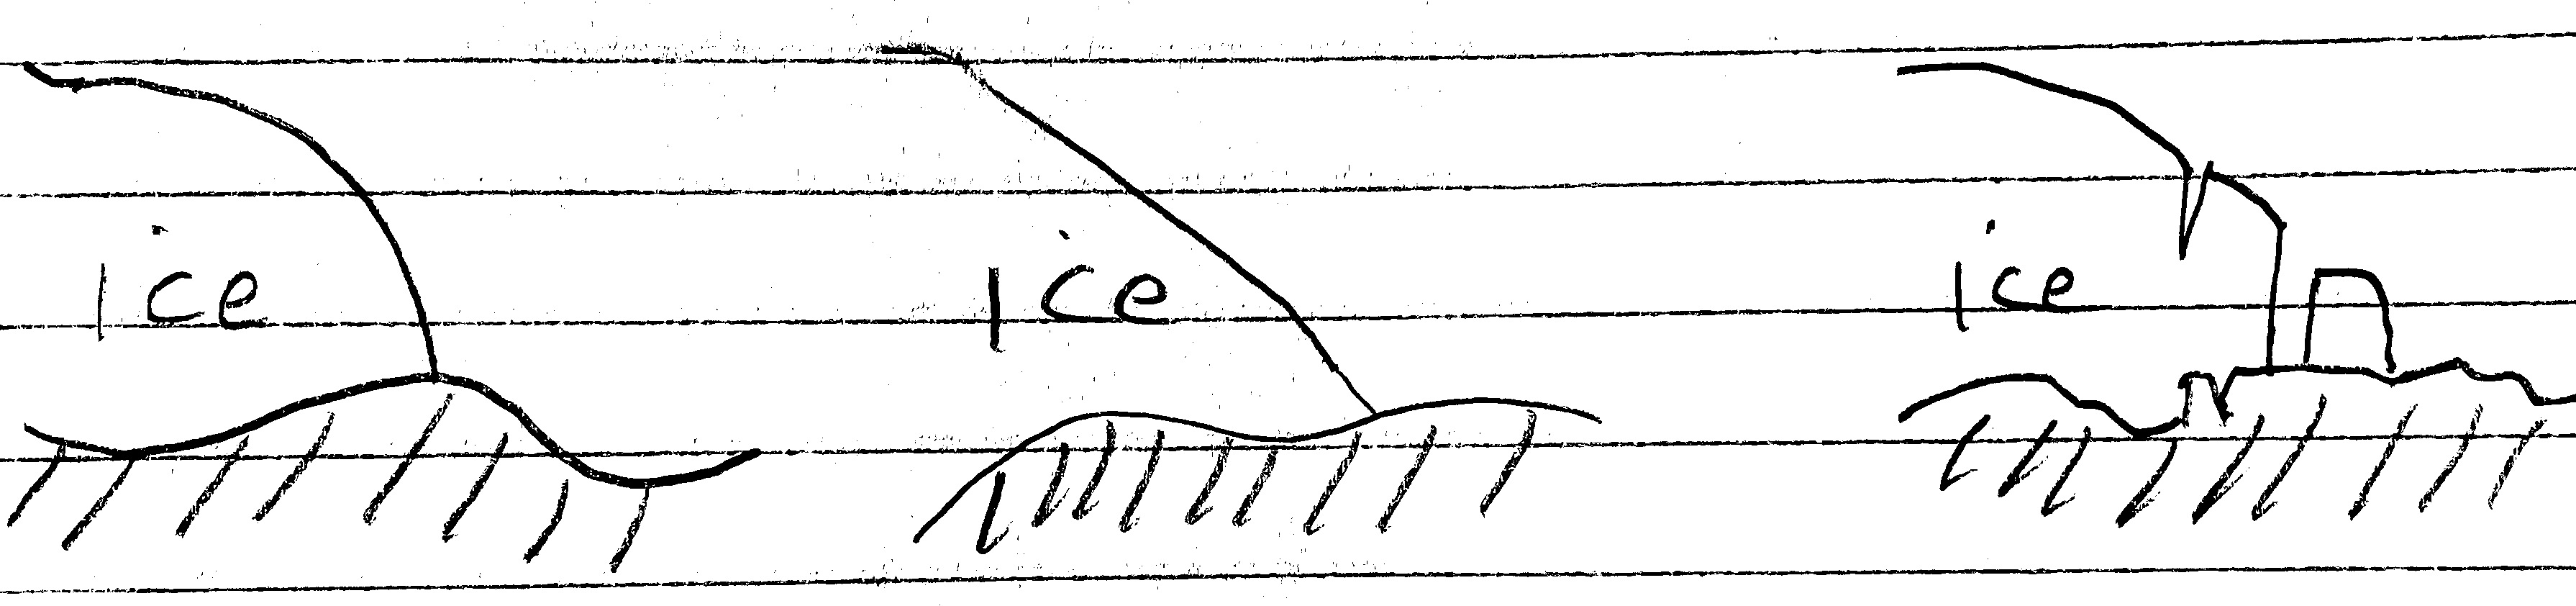
\includegraphics[width=0.8\textwidth]{figs/margins.jpg}
\end{center}
\caption{FIXME REDRAW.  In which Sobolev space should we seek the surface elevation function?  This question relates to the theoretically-expected shape of the ice margin.  The shallow ice theory yields a fractional power shape (left).  Other glacier models hypothesize a ``wedge'' shape (center).  On the other hand, actual glacier margins often have overhangs, crevasses, and cliffs (right).}
\label{fig:margins}
\end{figure}

Reality is of course more complicated.  In the vicinity of a steep ice margin, especially on steep bedrock features, real glacier ice can generate overhangs which violate the assumption of a single-valued surface elevation function.  Similarly, real bedrock can overhang.  Fractures, crevasses, and cliffs are commonly found in glacier margins, but modeling such features requires a departure from the viscous fluid paradigm considered here.
  
Because margins are small features compared to the overall scale of glaciers and ice sheets, most modeling literature ignores overhangs and assumes instead that surface and bed elevation functions are well-defined; see \cite{IsaacStadlerGhattas2015,Jouvetetal2008,LofgrenAhlkronaHelanow2022,WirbelJarosch2020} among many examples.  Extending Stokes-based viscous models by allowing overhangs, for example by supplementing momentum conservation with an additional advected damage variable \cite{PralongFunk2005}, so that ice-cliff calving can occur via a stress-failure criterion, might suggest mechanisms which explain how well-defined, integrable-gradient surface elevation functions arise as solutions to the kind of models considered in this paper.

\subsection{Conjectural well-posedness for the continuum problem} \label{subsec:conjecture} Subsections \ref{subsec:explicit}--\ref{subsec:margin} have deployed various imperfect arguments to explain why the backward Euler VI problem \eqref{eq:be:vi} could be well-posed, or why other approaches are less promising.  We now state a mathematically-precise conjectural framework for well-posedness of this problem based upon the idea that the surface motion map $\Phi(s) = -\bu|_s\cdot \bn_s$ assigns different results to inputs which differ in Sobolev norm, and indeed that it does so in a consistently and appropriately signed manner.

\begin{conjecture} \label{conj:b}  For $\rr>2$ such that Conjecture \ref{conj:a} holds, let $\cX = W^{1,\rr}(\Omega)$.  Fix $b\in\cX$ and let $\cK=\{r\in\cX\,:\,r|_{\partial\Omega}=b|_{\partial\Omega} \text{ and } r\ge b\}$.  Recall $\Phi:\cK\to\cX'$ is then well-defined by Lemma \ref{lem:philipschitz}.  Then there are constants $\alpha>0$ and $\qq>1$ so that
\begin{equation}
\left(\Phi(r) - \Phi(s)\right)[r-s] \ge \alpha \|r-s\|_{\cX}^\qq \qquad \text{for all } r,s\in\cK. \label{eq:conj:b}
\end{equation}
\end{conjecture}

Inequality \eqref{eq:conj:b} is called $\qq$-\emph{coercivity} of $\Phi$ over $\cK$.  In the abstract VI context of Section \ref{sec:abstractestimate}, if $F_{\Delta t}$ is both Lipschitz continuous (Lemma \ref{lem:philipschitz}) and $\qq$-coercive, over a closed and convex subset $\cK$ of a Banach space $\cX$, then \eqref{eq:be:vi} is well-posed.  This is what we prove next, namely that Conjectures \ref{conj:a} and \ref{conj:b} are sufficient for well-posedness of each implicit time step VI problem \eqref{eq:be:vi}.

\begin{theorem} \label{thm:stepwellposed}  Assume Conjectures \ref{conj:a} and \ref{conj:b}, and fix $b \in \cX$ to define $\cK$.  Suppose that $s^{n-1}\in\cK$ and that the SMB function $a(t,x)$ is in $C([0,T]; L^{\rr'}(\Omega))$.  Then there exists a unique surface elevation $s\in\cK$ satisfying backwards Euler VI problem \eqref{eq:be:vi}. \end{theorem}

\begin{proof}  Let $R>0$.  By Lemma \ref{lem:philipschitz} there is $C(R)>0$ so that if $r,s\in B_R\cap\cK$ then $\big|\Phi(r)[q] - \Phi(s)[q]\big| \le C(R) \|r-s\|_{\cX} \|q\|_{\cX}$.  Then by definition \eqref{eq:be:Fdefine}, H\"older's inequality, and Sobolev's inequality we have
\begin{align}
\left|F_{\Delta t}(r)[q] - F_{\Delta t}(s)[q]\right| &\le \int_\Omega |r-s||q| + \Delta t\, \big|\Phi(r)[q] - \Phi(s)[q]\big| \\
    &\le C \|r-s\|_{\cX} \|q\|_\cX \notag
\end{align}
for some $C>0$ which depends on $R$ and $\Delta t$.  Thus $F_{\Delta t}$ is (Lipschitz) continuous on bounded subsets of $\cK$.  If Conjecture \ref{conj:b} holds then
\begin{align}
\left(F_{\Delta t}(r) - F_{\Delta t}(s)\right)[r-s] &= \int_\Omega (r-s)^2 + \Delta t\, \left(\Phi(r) - \Phi(s)\right)[r-s] \\
    &\ge \alpha\Delta t \|r-s\|_{\cX}^\qq, \notag
\end{align}
so $F_{\Delta t}$ is $\qq$-coercive over $\cX$.  From definition \eqref{eq:be:source}, the hypothesis on $a$, and H\"older's inequality,
\begin{equation}
\big|\ell^n[q]\big| \le \left(\|s^{n-1}\|_{L^{\rr'}} + \Delta t \max_{t\in[t_{n-1},t_n]} \|a(t,\cdot)\|_{L^{\rr'}}\right) \|q\|_{L^\rr}
\label{eq:sourcetermbound}
\end{equation}
for all $q \in \cX$.  Because $\|s^{n-1}\|_{L^{\rr'}}<\infty$ by Sobolev's inequality, and $\|q\|_{L^\rr} \le \|q\|_{\cX}$, it follows that $\ell^n \in \cX'$.  Because $F_{\Delta t}$ is $\qq$-coercive it is also coercive and strictly-monotone (Definition \ref{def:monotonecoercive}).  Now Corollary III.1.8 of \cite{KinderlehrerStampacchia1980} shows existence of a solution to \eqref{eq:be:vi}, which is unique by strict monotonicity.
\end{proof}

Observe that Theorem \ref{thm:stepwellposed} addresses only the well-posedness of a single time-step problem over $[t_{n-1},t_n]$.  Its conclusion is not sufficient to show well-posedness of the time-dependent problem parabolic VI problem, over $[0,T]$, corresponding to NCP \eqref{eq:ncp}.  If this problem were known to be well-posed then one might analyze whether implicit steps converge in the $\Delta t\to 0$ limit.

The computation of $\bu|_s$ and $\Phi(s)=-\bu|_s\cdot \bn_s$, or equivalent expressions, would seem to be necessary in any evolving-geometry Stokes framework, and only these expressions are addressed in the Conjectures.  It would seem that those modeling practitioners who use Stokes dynamics expect Conjectures \ref{conj:a} and \ref{conj:b} to hold, or similar facts, but such may be difficult to prove despite some progress in Sections \ref{sec:stokes} and \ref{sec:model}.  Greater progress has been made in the SIA case \cite{Calvoetal2003,JouvetBueler2012,PiersantiTemam2023}, which might be helpful.  In any case, the geometry error bounds and results in the next two Sections only require the conclusion of Theorem \ref{thm:stepwellposed}, and not Conjectures \ref{conj:a} or \ref{conj:b} separately.


\section{Numerical evaluation of coercivity} \label{sec:numerical}

We may explore the validity of Conjecture \ref{conj:b} by sampling from numerical simulations.  The experiment here,\footnote{The source code at \href{https://github.com/bueler/glacier-fe-estimate}{\texttt{github.com/bueler/glacier-fe-estimate}} addresses all remaining details.} performed using Python and the Firedrake FE library \cite{Hametal2023}, is not intended to demonstrate implicit time-stepping, but only to generate admissible surface elevation pairs $r,s\in\cK$ to use as samples.  For a given sample pair we evaluate the coercivity ratio
\begin{equation}
\rho(r,s) = \frac{\left(\Phi(r) - \Phi(s)\right)[r-s]}{\|r-s\|_{\cX}^2}. \label{eq:Phiratio}
\end{equation}
If, for all pairs in some $\cK$, the set of ratios $\{\rho(r,s)\}$ were bounded below by a positive constant $\alpha>0$, then this would confirm the $\qq=2$ coercivity inequality \eqref{eq:conj:b} for that $\cK$.  Of course, a numerical experiment allows only finite sampling, and furthermore a finite discretization must be used so we cannot directly address the continuum set $\cK$.

The domain for our experiment is the 1D interval $\Omega=(-L,L)$, $L=100$ km, with $\cX = W_b^{1,2}(\Omega)$.  Three bed profiles  (Figure \ref{fig:cases}) were considered, \emph{flat} with $b=0$, \emph{smooth} with a superposition of several wavelengths down to 10 km, and \emph{rough} with an additional 4 km wavelength mode.  These beds generate corresponding constraint sets $\cK_i \subset \cX$, $i=1,2,3$.

\begin{figure}[ht]
\mbox{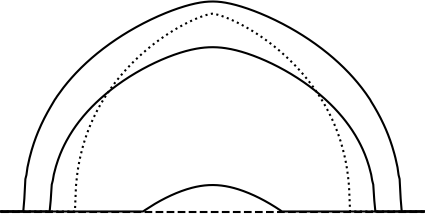
\includegraphics[width=0.31\textwidth]{figs/snapsflat.png} \, 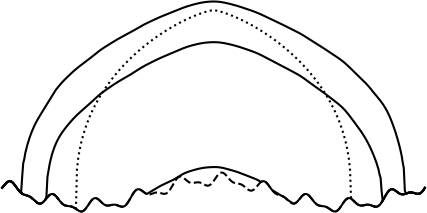
\includegraphics[width=0.335\textwidth]{figs/snapssmooth.png} \, 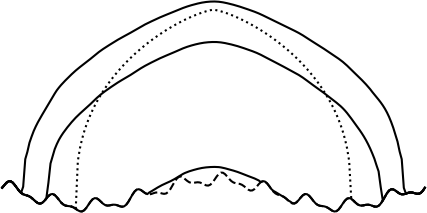
\includegraphics[width=0.335\textwidth]{figs/snapsrough.png}}

\caption{Three bed cases (flat, smooth, rough) define constraint sets $\cK_i\subset\cX$ in the numerical experiment.  For each $\cK_i$, three time-dependent runs of $T=200$ years, starting from the same initial state (dotted), but using different constant values of the SMB (see text), generated a large number of admissible states.  Example states at $t=170$ years are shown (solid).  Ratios \eqref{eq:Phiratio} were computed for 1000 sample pairs $r,s$ from each set $\cK_i$.}
\label{fig:cases}
\end{figure}

The interval $\Omega$ was uniformly-meshed into equal intervals.  The $P_1$ piecewise-linear FE space $\cX_h\subset \cX$ was used for the bed $b$ and the surface $s$, giving polygonal domains $\Lambda$ defined by $b,s$; see equation \eqref{eq:icydomain}.  The Stokes problem \eqref{eq:glenstokes:weak}, with viscosity regularization $\eps=10^{-19}\, \text{s}^{-2}$ in \eqref{eq:glen}, was solved on each domain $\Lambda$ using a vertically-extruded mesh of quadrilaterals (Figure \ref{fig:fe:operatorvisualization}), mixed FE method for the $Q_2\times Q_1$ (Taylor-Hood) stable pair \cite{Elmanetal2014}, and a Newton solver, with direct solution of the linear step equations.

For each constraint set $\cK_i$, three constant SMB values were considered (units $\text{m}\,\text{s}^{-1}$): $a=\{-2.5,0.0,1.0\}\times 10^{-7}$.  For each SMB value a time-dependent run of duration $T=200$ years started from the same initial surface elevation profile.\footnote{A Halfar profile \cite{Halfar1981} with characteristic time $t_0=29$ years was used as the initial state.  Thus, in the case of a flat bed and $a=0$ the exact time-dependent solution under SIA dynamics is known by Halfar's result \cite{Halfar1981}.  The final ($t=200$ a) surface elevation, computed using Stokes dynamics in the actual experiment, agrees closely with the SIA exact solution; compare comments in \cite{LofgrenAhlkronaHelanow2022}.}  The positive SMB value was sufficient to advance the ice margins nearly to the domain boundary at $|x|=L$ by the final time $t=200$ a, while the negative SMB value caused the glacier to disappear entirely by the final time.

In these simulations each time-step VI \eqref{eq:be:vi} was semi-implicit.  That is, definition \eqref{eq:be:Fdefine} was modified by using the prior surface velocity $\bu|_{s^{n-1}}$.  The numerical solution was by a reduced-space Newton method with line search, modified for VI application \cite{BensonMunson2006}.  The ``FSSA'' stabilization technique from \cite{LofgrenAhlkronaHelanow2022} was applied, which generates a modified Stokes weak form compared to \eqref{eq:glenstokes:weak}; see equation (23) in \cite{LofgrenAhlkronaHelanow2022}.  The resulting time-dependent numerical method is only conditionally stable, but adequate for the experimental purposes of generating sample surfaces.

The basic result of this experiment is shown in Figure \ref{fig:ratios}.  These are sample ratio $\rho(r,s)$ histograms from the highest spatial resolution, namely $\Delta x=500$ m and 40 elements in each extruded column.  More than $87\%$ of all the ratios were positive, and of these the medians for the three $\cK_i$ were in the range $[4.5,5.2] \times 10^{-13}$.  For the remaining negative ratios, the medians were in the range $[-4.1,-2.8]\times 10^{-14}$, much smaller in magnitude.

\begin{figure}[ht]
\mbox{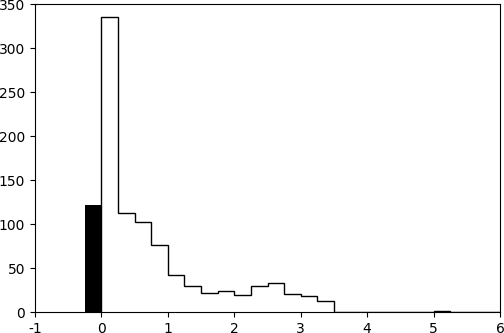
\includegraphics[width=0.33\textwidth]{figs/flatratios.png} \, 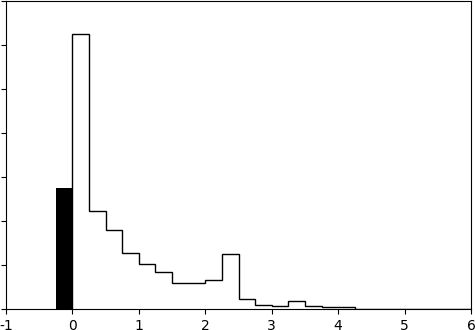
\includegraphics[width=0.31\textwidth]{figs/smoothratios.png} \, 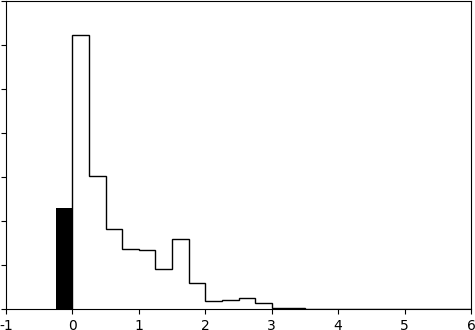
\includegraphics[width=0.31\textwidth]{figs/roughratios.png}}

\caption{Histograms of the equation \eqref{eq:Phiratio} ratios $\rho(r,s)$, for 1000 sample pairs from each of the same 3 sets $\cK_i$ in Figure \ref{fig:cases}.  The horizontal axis has  $\rho(r,s) \in [-1,6]\times 10^{-12}$, and the common vertical axis is for counts between 0 and 350.  About $10\%$ of these ratios are negative (solid).}
\label{fig:ratios}
\end{figure}

Figure \ref{fig:ratios} does \emph{not} represent compelling evidence of $2$-coercivity by definition \eqref{eq:qcoercive}, but it does not exclude it.  The discretization of the ice margin seemed to cause the negative ratios.  For example, noting that ratio evaluation uses integral \eqref{eq:definePhi}, if that integrand is reset to zero where the ice is thinner than 100 m then the negative values disappear (not shown).  Even without such thresholding, at lower horizontal resolution ($\Delta x=2000$ m), while the fraction of negative ratios was comparable, their median magnitude was roughly twice as large.  Thus the disappearance of negative ratios under grid refinement cannot be excluded.  Margin approximation improvements, such as adaptive/local mesh refinement, might also improve the numerical evidence for coercivity.

It is theoretically possible that the operator $\Phi$ is monotone (inequality \ref{eq:monotone}) but not $\qq$-coercive for any $\qq$.  In that case a revised well-posedness argument could be attempted, for example by adding a small coercive form as in section III.2 of \cite{KinderlehrerStampacchia1980}.

If a continuum pair $r,s$ with a negative ratio was actually found in some $\cK$, i.e.~with an exact continuum ratio $\rho(r,s)<0$ from \eqref{eq:Phiratio}, then the coercivity-based well-posedness framework of this paper would fail.  However, noting that real glaciers appear to evolve deterministically, and given that real glaciers experience substantial fracturing at margins (e.g.~Figure \ref{fig:margins}), it is possible that a more-complete physical model, perhaps including non-fluid processes like fractures, would permit coercivity of the corresponding $\Phi$ operator.

Regarding Conjecture \ref{conj:a}, i.e.~Lipschitz continuity for surface velocity traces, the maximum ratio $\big\|\bu|_r - \bu|_s\big\|_{L^2}/\|r-s\|_{W^{1,2}}$ for the same sample pairs was also evaluated.  Over all three sets $\cK_i$, computed at the highest resolution ($500$ m), the maximum ratio was $3.5\times 10^{-9}$, providing a lower bound for $C_A$.  Again, numerical experiments obviously cannot prove the Conjecture.


\section{Abstract error estimate for a finite element approximation} \label{sec:abstractestimate}

In this Section we consider the finite element (FE) approximation of an abstract variational inequality (VI) problem.  We will return to glaciological problem \eqref{eq:be:vi} in Section \ref{sec:application}.

Let $\cX$ be a real reflexive Banach space with norm $\|\cdot\|$ and topological dual (Banach) space $\cX'$.  Denote the dual pairing of $\ell \in \cX'$ and $v\in\cX$ by $\ell[v]$, and define $\|\ell\|_{\cX'} = \sup_{\|v\|=1} \big|\ell[v]\big|$.  Let $\cK \subset \cX$ be a nonempty, closed, and convex subset, called the constraint set, whose elements are called admissible.  For a continuous, but generally nonlinear, operator $f:\cK \to \cX'$, and a source $\ell\in \cX'$, the VI problem is to find $u\in \cK$ such that
\begin{equation}
f(u)[v-u] \ge \ell[v-u] \quad \text{for all } v\in \cK. \label{eq:vi}
\end{equation}
The best known example of such a problem is the obstacle problem for the Laplacian operator---see \cite{Ciarlet2002,Evans2010,KinderlehrerStampacchia1980} for theory and FE analysis, and VI \eqref{eq:be:vi} is in this form.  A key observation is that $f(u)-\ell \in \cX'$ is generally nonzero when $u$ solves \eqref{eq:vi}, though if $u$ is in the interior of $\cK$ then $f(u)=\ell$.  Under sufficient regularity assumptions an NCP like \eqref{eq:ncp} or \eqref{eq:be:ncp} follows from \eqref{eq:vi}.

The following definitions are standard \cite[Chapter III]{KinderlehrerStampacchia1980}.  The definition of $\qq$-coercive appeared in Conjecture \ref{conj:b}.

\begin{definition} \label{def:monotonecoercive}
An operator $f:\cK \to \cX'$ is said to be \emph{monotone} if
\begin{equation}
\left(f(v)-f(w)\right)[v-w] \ge 0 \qquad \text{for all } v,w \in \cK \label{eq:monotone}
\end{equation}
and \emph{strictly monotone} if equality in \eqref{eq:monotone} implies $v=w$.  It is \emph{coercive} if there is $w\in \cK$ so that $\left(f(v)-f(w)\right)[v-w]/\|v-w\| \to +\infty$ for $v \in \cK$ as $\|v\| \to +\infty$.  It is \emph{$\qq$-coercive} \cite{Bueler2021conservation}, for some $\qq>1$, if there exists $\alpha>0$ such that
\begin{equation}
\left(f(v)-f(w)\right)[v-w] \ge \alpha \|v-w\|^\qq \qquad \text{for all } v,w \in \cK. \label{eq:qcoercive}
\end{equation}
\end{definition}

If $f:\cK \to \cX'$ is monotone and coercive, and also continuous on finite-dimensional subspaces, then VI \eqref{eq:vi} has a solution \cite[Corollary III.1.8]{KinderlehrerStampacchia1980}.  If $f$ is strictly monotone then the solution is unique.  If $f$ is $\qq$-coercive then it coercive and strictly monotone, so $\qq$-coercivity and continuity yield well-posedness for \eqref{eq:vi}.  Note that Definitions \ref{def:monotonecoercive} and \ref{def:lipshitz} do not require $f$ to be defined on all of $\cX$, but only on $\cK$.  
  
The following definition appeared in Lemma \ref{lem:philipschitz}.  If it holds then $f$ is continuous.

\begin{definition} \label{def:lipshitz}
For $R>0$ let $B_R = \{v\in \cX\,:\,\|v\|\le R\}$.  We say $f:\cK \to \cX'$ is \emph{Lipshitz on bounded subsets of $\cK$} if for every $R>0$ there is $C(R)>0$ so that if $v,w \in B_R \cap \cK$ and $z\in\cX$ then $|\left(f(v)-f(w)\right)[z]| \le C(R) \|v-w\| \|z\|$, equivalently
\begin{equation}
\|f(v)-f(w)\|_{\cX'} \le C(R) \|v-w\| \quad \text{ for all } v,w \in B_R \cap \cK.  \label{eq:liponbounded}
\end{equation}
\end{definition}

An FE method for \eqref{eq:vi} is a finite-dimensional VI problem.  Suppose $\cX_h \subset \cX$ is a finite-dimensional subspace, typically some space of continuous, piecewise-polynomial functions defined on a mesh.  The FE constraint set $\cK_h\subset \cX_h$ is assumed to be closed and convex, but generally $\cK_h \nsubseteq \cK$.  Let $f_h:\cK_h\to\cX'$, and note that generally $f_h\ne f$ because of quadrature and other approximations.  (Looking ahead, both $\cK_h \nsubseteq \cK$ and $f_h\ne f$ occur naturally in the glacier geometry problem; see Section \ref{sec:application}.)  The FE VI problem is
\begin{equation}
f_h(u_h)[v_h-u_h] \ge \ell[v_h-u_h] \quad \text{for all } v_h\in \cK_h. \label{eq:fe:vi}
\end{equation}
We will assume that \eqref{eq:fe:vi} has a solution $u_h\in\cK_h$.

The following abstract error estimation theorem extends the well-known result by Falk \cite{Falk1974}; see also Theorem 5.1.1 in \cite{Ciarlet2002}.  We will \emph{not} assume and of the following: $f$ is linear, $\cK_h \subset \cK$, $f_h=f$, $f_h$ is $\qq$-coercive, $f$ is Lipschitz, or $f_h$ is continuous.  However, we must assume that the domain of $f$ includes the FE solution, which is achieved here by defining a convex superset of $\cK$ and $\cK_h$.  This technical assumption permits a clean and general estimation theorem, but the choice of $\cK_h$ made in Section \ref{sec:application} means that $\hcK$ is not needed in our glacier application; see Corollary \ref{cor:abstractestimate:nohull}.

\begin{theorem} \label{thm:abstractestimate}  Define $\hcK = \overline{\Hull{(\cK \cup \cK_h)}}$ as the closure in $\cX$ of the convex hull of $\cK \cup \cK_h$, and suppose that $f:\hcK \to \cX'$.  For $\qq>1$, with conjugate exponent $\qq'=\qq/(\qq-1)$, assume that $f$ is $\qq$-coercive over $\hcK$ with constant $\alpha>0$, and Lipshitz on bounded sets of $\hcK$.  Suppose $u\in\cK$ solves \eqref{eq:vi} and $u_h\in\cK_h$ solves \eqref{eq:fe:vi}, and let $R_h=\max\{\|u\|,\|u_h\|\}$.  Then there is a constant $c=c(R_h)>0$, not otherwise depending on $u$ or $u_h$, so that
\begin{align}
\|u-u_h\|^\qq &\le \quad \frac{2}{\alpha} \inf_{v\in\cK} \left(f(u)-\ell\right)[v-u_h] \label{eq:abstractestimate} \\
   &\quad\, + \frac{2}{\alpha} \inf_{v_h\in\cK_h} \left(f(u)-\ell\right)[v_h-u] \notag \\
   &\quad\, + \frac{2}{\alpha} \left(f(u_h)-f_h(u_h)\right)[u_h] \notag \\
   &\quad\, + \inf_{v_h\in\cK_h} c \|v_h - u\|^{\qq'}. \notag
\end{align}
\end{theorem}

\begin{proof}  For arbitrary $v\in\cK$ and $v_h\in\cK_h$, rewrite \eqref{eq:vi} and \eqref{eq:fe:vi} as follows:
\begin{align}
f(u)[u]     &\le f(u)[v] + \ell[u-v], \label{eq:abstract:one}  \\
f_h(u_h)[u_h] &\le f_h(u_h)[v_h] + \ell[u_h-v_h]. \notag
\end{align}
It follows from \eqref{eq:abstract:one} and the $\qq$-coercivity of $f$ that
\begin{align}
\alpha \|u-u_h\|^\qq &\le \left(f(u)-f(u_h)\right)[u-u_h] \label{eq:abstract:two} \\
  &= f(u)[u] + f(u_h)[u_h] - f(u)[u_h] - f(u_h)[u] \notag \\
  &= f(u)[u] + f_h(u_h)[u_h] \notag \\
  &\qquad - f(u)[u_h] - f(u_h)[u] + \left(f(u_h)-f_h(u_h)\right)[u_h] \notag \\
  &\le f(u)[v] + \ell[u-v] + f(u_h)[v_h] + \ell[u_h-v_h] \notag \\
  &\qquad - f(u)[u_h] - f(u_h)[u] + \left(f(u_h)-f_h(u_h)\right)[u_h] \notag \\
  &= f(u)[v-u_h] - \ell[v-u_h] + f(u_h)[v_h-u] - \ell[v_h-u] \notag \\
  &\qquad + \left(f(u_h)-f_h(u_h)\right)[u_h] \notag \\
  &= \left(f(u)-\ell\right)[v-u_h] + \left(f(u)-\ell\right)[v_h-u] \notag \\
  &\qquad + \left(f(u)-f(u_h)\right)[u-v_h] + \left(f(u_h)-f_h(u_h)\right)[u_h] \notag
\end{align}
Since $u,u_h\in B_{R_h}$, by the Lipshitz assumption over $\hcK$ there is $C(R_h)>0$ so that
\begin{equation}
\left(f(u)-f(u_h)\right)[u-v_h] \le C(R_h) \|u-u_h\|\|u-v_h\|. \label{eq:abstract:three}
\end{equation}
Noting $1<\qq<\infty$, now use Young's inequality with $\eps>0$ \cite[Appendix B.2]{Evans2010}:
\begin{align}
\alpha \|u-u_h\|^\qq &\le \left(f(u)-\ell\right)[v-u_h] + \left(f(u)-\ell\right)[v_h-u]  \label{eq:abstract:four} \\
  &\qquad + C(R_h) \left(\eps\|u-u_h\|^\qq + \tilde C(\eps) \|u-v_h\|^{\qq'}\right) \notag \\
  &\qquad + \left(f(u_h)-f_h(u_h)\right)[u_h], \notag
\end{align}
where $\tilde C(\eps) = (\eps \qq)^{-\qq'/\qq} {\qq'}^{-1}$.  Choose $\eps>0$ so that $C(R_h) \eps \le \alpha/2$, and subtract:
\begin{align}
\frac{\alpha}{2} \|u-u_h\|^\qq &\le \left(f(u)-\ell\right)[v-u_h] + \left(f(u)-\ell\right)[v_h-u]  \label{eq:abstract:five} \\
  &\qquad + C(R_h) \tilde C(\eps) \|u-v_h\|^{\qq'} + \left(f(u_h)-f_h(u_h)\right)[u_h] \notag
\end{align}
Take infimums to show \eqref{eq:abstractestimate}.
\end{proof}

The next Corollary addresses two important cases where the convex hull operation is not needed.  We will see in Section \ref{sec:application} that case \emph{i)} can be imposed in glacier simulations.

\begin{corollary}  \label{cor:abstractestimate:nohull}  In addition to the assumptions of Theorem \ref{thm:abstractestimate}, suppose that one of the following situations apply:
\renewcommand{\labelenumi}{\roman{enumi})}
\begin{enumerate}
\item $\cK_h \subset \cK$, with $f$ $\qq$-coercive over $\cK$, or
\item $f$ is defined on, and $\qq$-coercive over, all of $\cX$.
\end{enumerate}
Then, without the construction of the convex hull $\hcK$, conclusion \eqref{eq:abstractestimate} applies as stated, and in case i) the ``\,$\inf_{v\in\cK}$'' term in \eqref{eq:abstractestimate} is zero.
\end{corollary}

Consider $f(u)-\ell\in \cX'$.  It might be a measure or a measurable function, and the first two terms in estimate \eqref{eq:abstractestimate} preserve information about its support.  (This plays a role in the glacier application of Section \ref{sec:application}.)  By contrast, the Hilbert space result in \cite{Falk1974} computes norms and loses this information.  The following Corollary, with easy proof, takes such a norm-based approach.  We suppose that $\cX$ continuously and densely embeds into a larger Banach space $\cB$:
\begin{equation}
\cX \hookrightarrow \cB, \quad \bar{\cX} = \cB \label{eq:VembedsinB}
\end{equation}
Observe that $\cB' \subset \cX'$.  A standard example is $\cX=W^{1,\rr}(\Omega)$ and $\cB=L^\rr(\Omega)$.

\begin{corollary}  \label{cor:abstractestimate:Bnorm}  In addition to the assumptions of Theorem \ref{thm:abstractestimate}, suppose \eqref{eq:VembedsinB} holds, and that $\|f(u)-\ell\|_{\cB'} < \infty$.  Then
\begin{align}
\|u-u_h\|^\qq &\le \frac{2}{\alpha} \|f(u)-\ell\|_{\cB'} \left( \inf_{v\in\cK} \|v-u_h\|_{\cB} +   \inf_{v_h\in\cK_h} \|v_h-u\|_{\cB} \right) \label{eq:abstractestimate:Bnorm} \\
   &\qquad + \frac{2}{\alpha} \left(f(u_h)-f_h(u_h)\right)[u_h] + \inf_{v_h\in\cK_h} c \|v_h - u\|^{\qq'} \notag
\end{align}
\end{corollary}

The result by Falk \cite{Falk1974} combines the above two Corollaries, under the further assumption that $f$ is linear.  To say this precisely, suppose $f(v)[w]=a(v,w)$ is bilinear, uniformly elliptic, and continuous on a Hilbert space $\cX$.  (The definition of uniformly elliptic coincides with definition \eqref{eq:qcoercive} of $2$-coercive, and continuity of $a(v,w)$ implies \eqref{eq:liponbounded}.)  Suppose that $\cX\hookrightarrow \cH$ and $\bar{\cX} = \cH$ for some Hilbert space $\cH$, and that $\|f(u)-\ell\|_{\cH'} < \infty$ so that, up to isomorphism, $f(u)-\ell \in \cH$.  Finally, suppose that $f(u_h)=f_h(u_h)$.  Then case \emph{ii)} of Corollary \ref{cor:abstractestimate:nohull} combines with Corollary \ref{cor:abstractestimate:Bnorm} to yield Theorem 1 in \cite{Falk1974}.

The $\inf_{v\in\cK}$ term in estimates \eqref{eq:abstractestimate} and \eqref{eq:abstractestimate:Bnorm} is generally nonzero in obstacle problems where $\cK_h \not\subset \cK$.  In fact, consider a unilateral obstacle problem where $\cK=\{v \in \cX\,:\,v\ge \psi\}$.  Suppose $\psi_h=\pi_h \psi$ is the FE interpolant of $\psi$, and define $\cK_h=\{v_h \in \cX_h\,:\,v_h\ge \psi_h\}$.  While $\psi_h(x_j)=\psi(x_j)$ for interpolation nodes $x_j$, generally $\psi_h(x) \ge \psi(x)$ may not hold for $x\in\Omega$ even if $\psi$ is arbitrarily smooth, nor $\psi_h(x) \le \psi(x)$.  Thus nodal admissiblity does not generally imply admissibility if interpolation is applied to the obstacle (Figure \ref{fig:nonadmissible}, left; see also \cite[Figure 5.1.3]{Ciarlet2002}).

\begin{figure}[ht]
\begin{center}
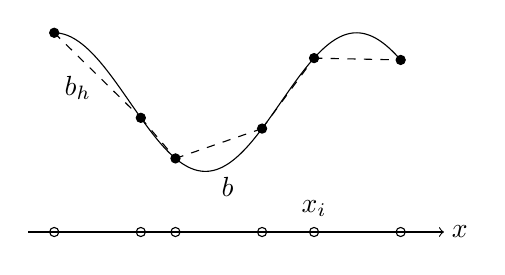
\begin{tikzpicture}[scale=1.1, domain=0.0:4.0, samples=200]
  \draw[black,thin,->] (-0.3,0.0) -- (4.5,0.0) node [xshift=2mm] {$x$};
  \draw plot (\x, {1.5 + 0.8 * cos(1.8*\x r)});
  \node[yshift=-2mm] at (2.0, 0.7) {$b$};
  \newcommand{\xlist}{0.0, 1.0, 1.4, 2.4, 3.0, 4.0}
  \foreach \x [remember=\x as \lastx] in \xlist {
      \draw (\x, 0.0) circle (1.5pt);
      \filldraw (\x, {1.5 + 0.8 * cos(1.8*\x r)}) circle (1.5pt);
      \draw[dashed] (\lastx, {1.5 + 0.8 * cos(1.8*\lastx r)}) -- (\x, {1.5 + 0.8 * cos(1.8*\x r)});
  }
  \node[yshift=3mm] at (3.0, 0.0) {$x_i$};
  \node[xshift=3mm, yshift=-7mm] at (0.0, 2.3) {$b_h$};
\end{tikzpicture}
 \quad 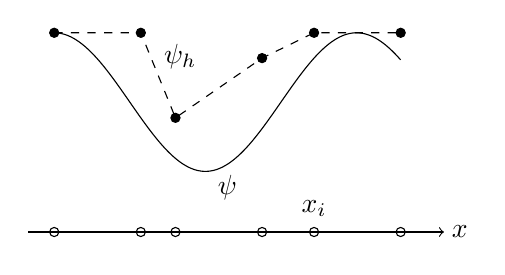
\begin{tikzpicture}[scale=1.1, domain=0.0:4.0, samples=200]
  \draw[black,thin,->] (-0.3,0.0) -- (4.5,0.0) node [xshift=2mm] {$x$};
  \draw plot (\x, {1.5 + 0.8 * cos(1.8*\x r)});
  \newcommand{\xlist}{0.0, 1.0, 1.4, 2.4, 3.0, 4.0}
  \newcommand{\xymaxlist}{0.0/2.3, 1.0/2.3, 1.4/1.3182, 2.4/2.0078, 3.0/2.3, 4.0/2.3}
  \foreach \x/\y in \xymaxlist {
      \draw (\x, 0.0) circle (1.5pt);
      \filldraw (\x, \y) circle (1.5pt);
  }
  \node[yshift=3mm] at (3.0, 0.0) {$x_i$};
  \draw[dashed] (0.0,2.3) -- (1.0,2.3) -- (1.4,1.3182) -- (2.4,2.0078) -- (3.0,2.3) -- (4.0,2.3);
  \node[yshift=-2mm] at (2.0, 0.7) {$\psi$};
  \node[xshift=5mm, yshift=-3mm] at (1.0, 2.3) {$\psi_h$};
\end{tikzpicture}

\end{center}
\caption{Left: If $\psi_h=\pi_h\psi$ is the interpolant of $\psi$ then generally $\cK_h\subset\cK$ will not hold.  (Nodal admissibility does not imply admissibility.)  Right: Generating the FE obstacle by $\psi_h=R^{\oplus} \psi \ge \psi$, using monotone nodal operator \eqref{eq:monotoneop}, implies $\cK_h\subset\cK$.}
\label{fig:nonadmissible}
\end{figure}

For glacier models which track the surface elevation, in Section \ref{sec:application} we propose to bypass the above issue using a one-sided interpolation process using a monotone nodal operator (Figure \ref{fig:nonadmissible}, right), defined as follows.  Assume $P_1$ elements and a continuous obstacle $\psi$.  For a given triangulation $\cT_h$ and node $x_i$ let
\begin{equation}
(R^{\oplus}\psi)(x_i) = \max_{x \in N_i} \psi(x), \label{eq:monotoneop}
\end{equation}
where $N_i$ is the closure of the union of the elements adjacent to $x_i$ \cite{BuelerFarrell2024}.  Let $\psi_h$ be the unique $P_1$ function with nodal values $(R^{\oplus}\psi)(x_i)$.

Observe that models which solve for ice thickness using $P_1$ elements intrinsically bypass the issue because then $\cK = \{v\in\cX\,:\,v\ge 0\}$ and $\cK_h=\cK\cap\cX_h \subset \cK$.

The following Corollary collects some conclusions one might draw from assuming $\cK_h \subset \cK$ and further assumptions, especially that $f_h=f$.  Note that \eqref{eq:abstractestimate:subset:Cea} is Cea's lemma \cite[Theorem 2.4.1]{Ciarlet2002} in a Banach space, though with a constant which depends on $R_h=\max\{\|u\|,\|u_h\|\}$.  This is the PDE case with no active set or free boundary, which applies in the glacier context only when the entire domain $\Omega$ is covered in ice.

\begin{corollary}  \label{cor:abstractestimate:various}  Make the assumptions of case i) of Corollary \ref{cor:abstractestimate:nohull}.  Also assume that $f_h(u_h)[u_h] = f(u_h)[u_h]$.  Then
\begin{equation}
\|u-u_h\|^\qq \le  \inf_{v_h\in\cK_h} \left\{\frac{2}{\alpha} \left(f(u)-\ell\right)[v_h-u] + c \|v_h - u\|^{\qq'}\right\}. \label{eq:abstractestimate:subset}
\end{equation}
If also the assumptions of Corollary \ref{cor:abstractestimate:Bnorm} hold then
\begin{equation}
\|u-u_h\|^\qq \le \inf_{v_h\in\cK_h} \left\{\frac{2}{\alpha} \|f(u)-\ell\|_{\cB'} \|v_h-u\|_{\cB} + c \|v_h-u\|^{\qq'}\right\} \label{eq:abstractestimate:subset:Bnorm}
\end{equation}
If $f(u)=\ell$, for example if $u$ is in the interior of $\cK$, then
\begin{equation}
\|u-u_h\|^\qq \le c \inf_{v_h\in\cK_h} \|v_h-u\|^{\qq'} \label{eq:abstractestimate:subset:Cea}
\end{equation}
\end{corollary}


\section{Application of the theory to numerical glacier models} \label{sec:application}

Now we can synthesize the theory and apply it to an implicit time step of a glacier simulation which uses Stokes dynamics.  This will give ``conforming FE method'' a precise meaning for evolving-geometry glacier simulations.  We will combine three types of results: \emph{i)} well-posedness theory and \emph{a priori} bounds for the glaciological Stokes problem on a fixed domain (Section \ref{sec:stokes}), \emph{ii)} conjectural well-posedness theory of the surface elevation VI problem (Sections \ref{sec:model} and \ref{sec:theory}), and \emph{iii)} an abstract error estimate for FE solutions of VIs (Section \ref{sec:abstractestimate}).

Consider an FE method for VI problem \eqref{eq:be:vi}.  For a finite-dimensional subspace $\cX_h\subset \cX$, with a constraint set $\cK_h\subset \cX_h$, we seek $s_h\in\cK_h$ solving
\begin{equation}
F^h_{\Delta t}(s_h)[r_h-s_h] \ge \ell^n[r_h-s_h] \quad \text{for all } r_h \in \cK_h. \label{eq:fe:be:vi}
\end{equation}
The operator $F^h_{\Delta t}$ denotes an FE approximation to the operator $F_{\Delta t}$ defined in \eqref{eq:be:Fdefine}, while $\ell^n = s^{n-1} + \Delta t\,a^n$ is defined exactly as before, by equation \eqref{eq:be:source}.  We assume that $s^{n-1} \in \cK$ is general, and not necessarily that it is in the FE space $\cK_h$.

Evaluation of $F^h_{\Delta t}(s_h)$ in the FE VI problem \eqref{eq:fe:be:vi} requires the nontrivial numerical solution of a glaciological Stokes problem \eqref{eq:stokes} over a 3D mesh of the domain between $z=b_h$ and $z=s_h$ (Figure \ref{fig:fe:operatorvisualization}).  Such a mesh need not be extruded vertically as shown, nor must $s_h$ necessarily be piecewise-linear, but the upper and lower surfaces, where boundary conditions \eqref{eq:stokes:stressfreesurface} and \eqref{eq:stokes:noslide} are applied, must be FE-space functions, i.e.~$s_h,b_h\in\cX_h$ with $s_h\ge b_h$.  The numerical velocity from solving the Stokes problem, over the domain geometry defined by $s_h$, is denoted $\bu_h$, and its surface trace is denoted $\bu_h|_{s_h}$.  Observe that $\bu_h|_{s_h}$ will generally be different from the surface trace of the exact solution of the same Stokes boundary value problem for the same ($s_h$) geometry, denoted by $\bu|_{s_h}$.  Although $F^h_{\Delta t}(s_h)$ is defined by formula \eqref{eq:be:Fdefine}, it is a different operator from $F_{\Delta t}(s_h)$ because it uses the numerical solution velocity and not the exact solution velocity (of the \emph{same} Stokes problem).

\begin{figure}[ht]
\begin{center}
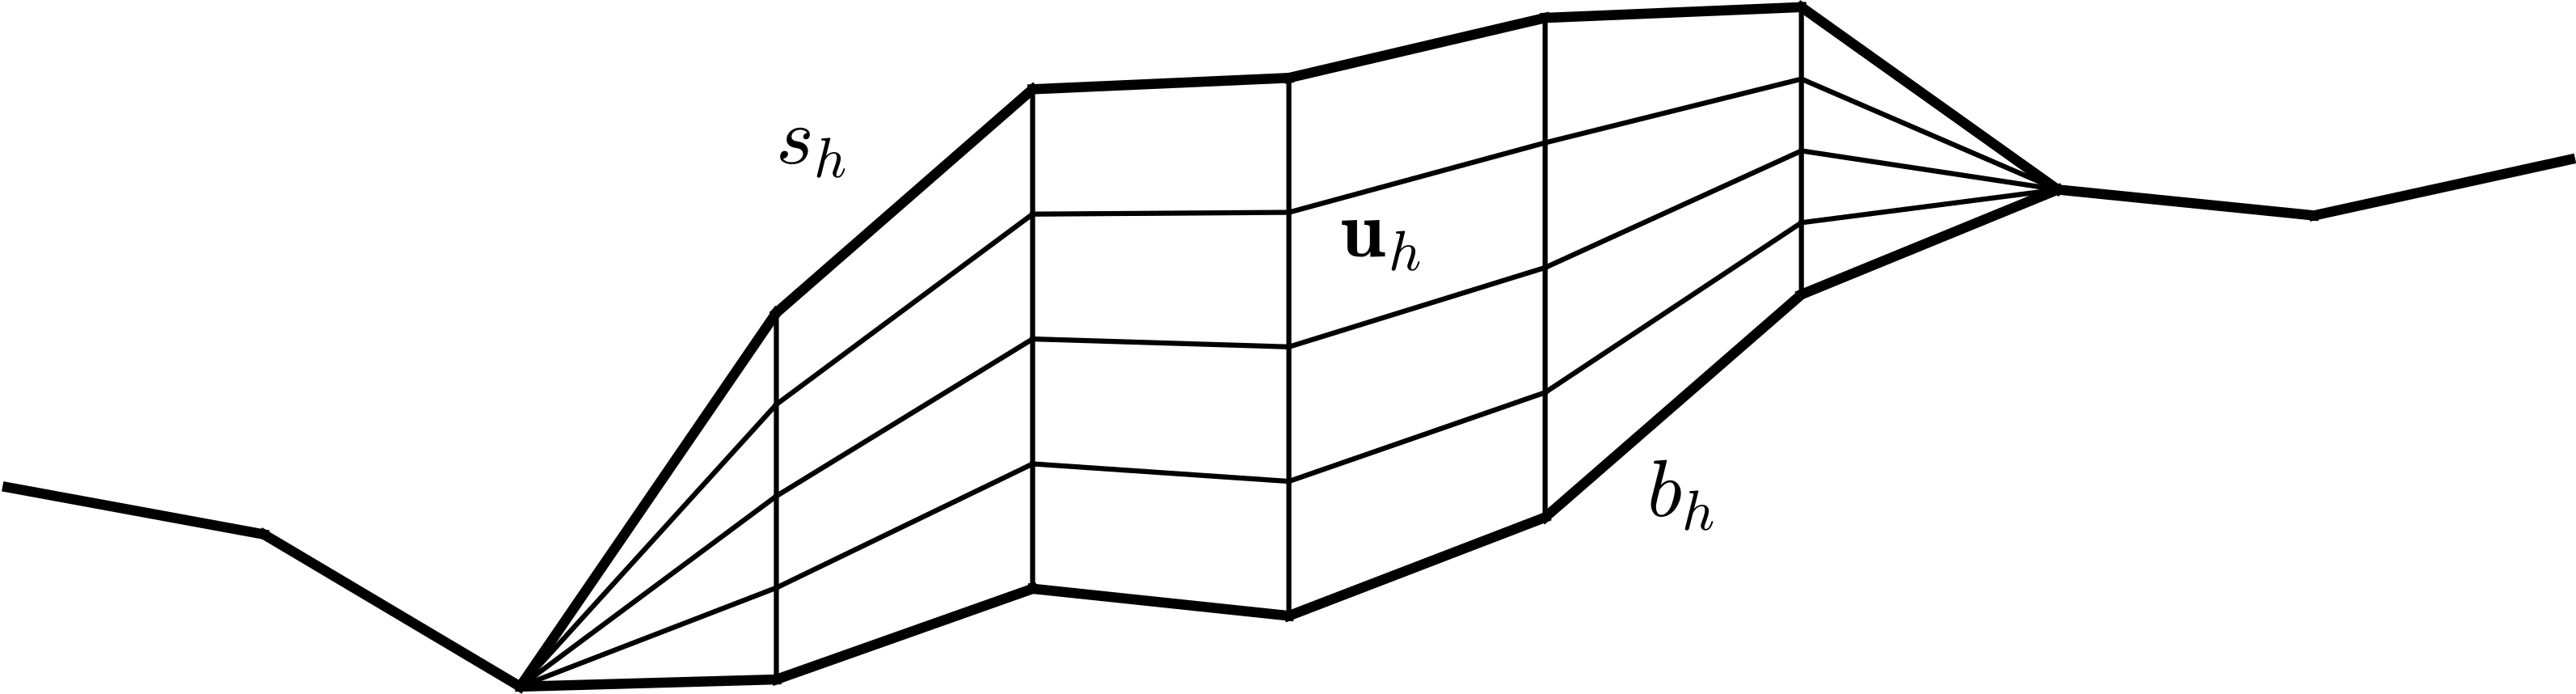
\includegraphics[width=0.75\textwidth]{genfigs/extruded.pdf}
\end{center}
\caption{Evaluating $F^h_{\Delta t}(s_h)$ in \eqref{eq:fe:be:vi} requires numerically solving a Stokes problem for velocity $\bu_h$, on a mesh between $b_h$ and $s_h$, and then evaluating its upper surface trace.}
\label{fig:fe:operatorvisualization}
\end{figure}

A key concern in applying abstract Theorem \ref{thm:abstractestimate} or its Corollaries in a glaciological context is the choice of the numerical bed elevation $b_h \approx b$, which defines the constraint set $\cK_h$.  We will assume $b$ is continuous on the closed domain $\bar\Omega$.  An abstract $b\in C(\bar\Omega) \cap \cX$ can be considered, but in practice $b$ is provided via a high resolution map derived from ice-penetrating radar \cite{Morlighemetal2017}.  It may already be in an FE space, but often on a (much) finer mesh.

Because of what we prove below, we assert that it is better to choose $b_h \in \cX_h$ to satisfy $b_h\ge b$.  A monotone nodal operator \eqref{eq:monotoneop}, or similar, can be applied, $b_h = R^\oplus b$.  As one would in ``conforming'' FE methods for PDE problems \cite{Elmanetal2014}, we assume $b_h=b$ along the fixed boundary $\partial\Omega$.

We define an interpolation and truncation operation $\Pi_h : \cX \to \cK_h$ as follows.  For $r\in\cX$ this gives the unique FE function $\Pi_h(r) \in \cX_h$ so that
\begin{equation}
\Pi_h(r)(x_j) = \max \,\{b_h(x_j), r(x_j)\} \label{eq:definePi}
\end{equation}
for every interior node $x_j \in \cT_h$, with $\Pi_h(x_j)=b(x_j)$ if $x_j\in\partial\Omega$.  Observe that definition \eqref{eq:definePi} only yields nodal admissibility.  The FE space must be such that this implies admissibility \emph{per se}, namely that $\Pi_h(r)(x) \ge b_h(x)$ for all $x \in \Omega$, so that $\Pi_h(r) \in \cK_h$.  This condition is satisfied by the continuous and piecewise-linear FE space $P_1$, but not, for example, by $P_2$ \cite{BuelerFarrell2024}, but compare the higher-order approach taken in \cite{KeithSurowiec2023}.

To summarize, from now on we make certain standard assumptions for solving VI problem \eqref{eq:be:vi} using numerical scheme \eqref{eq:fe:be:vi}.

\smallskip
\begin{assumptions}
The following data are given:
\begin{enumerate}
\item A bounded, convex polygon $\Omega\subset\RR^2$.
\item An exponent $\rr > 2$, with conjugate exponent $\rr' = \rr/(\rr-1)$. \label{item:rr}
\item A time-dependent SMB function $a\in C([0,T]; L^{\rr'}(\Omega))$.
\item A bed topography function $b \in C(\bar\Omega) \cap W^{1,\rr}(\Omega)$, with piecewise-linear boundary values $b|_{\partial\Omega}$.
\end{enumerate}
We make these definitions:
\begin{enumerate}
\setcounter{enumi}{4}
\item $\cX = W^{1,\rr}(\Omega)$, with the norm as defined in \eqref{eq:norm:Omega}.
\item $\cK = \{r\in\cX\,:\,r|_{\partial \Omega} = b|_{\partial \Omega} \text{ and } r \ge b\}$.
\item $\cX_h \subset \cX$ denotes a finite-dimensional and conforming FE space, from a mesh $\cT_h$ exactly tiling $\bar\Omega$.
\item The boundary values $b|_{\partial\Omega}$ are exactly representable in the FE space.
\end{enumerate}
The following are assumed to hold:
\begin{enumerate}
\setcounter{enumi}{8}
\item Conjecture \ref{conj:a} holds with Lipschitz constant $\CA > 0$. \label{item:conj:a}
\item Conjecture \ref{conj:b} holds with exponent $\qq>1$ and coercivity constant $\alpha > 0$.\label{item:conj:b}
\end{enumerate}
We also assume and define:
\begin{enumerate}
\setcounter{enumi}{10}
\item $b_h\in\cX_h$ is given, with $b_h\ge b$ on $\bar\Omega$ and $b_h=b$ along $\partial \Omega$. \label{item:goodbh}
\item $\cK_h = \{r_h\in\cX_h\,:\,r_h|_{\partial \Omega} = b_h|_{\partial \Omega} \text{ and } r_h \ge b_h\}$. \label{item:defineKh}
\item Interpolation/truncation $\Pi_h$ yields admissible elements in $\cK_h$.  \label{item:Pi}
\end{enumerate}
\end{assumptions}

\medskip
The conforming condition $\cK_h\subset \cK$ follows from assumptions \ref{item:goodbh} and \ref{item:defineKh}, with advantages to be exposed.  As seen in the proof of Theorem \ref{thm:stepwellposed}, assumptions \ref{item:conj:a} and \ref{item:conj:b} show that $F_{\Delta t}$ is $\qq$-coercive and Lipschitz on bounded subsets of $\cK$.  By Theorem \ref{thm:stepwellposed} and case \emph{i)} of Corollary \ref{cor:abstractestimate:nohull} we have the following Lemma.

\begin{lemma} \label{lem:preglacierapp}  Make the Standard Assumptions.  Suppose that $s^{n-1}\in\cK$ and define $\ell^n \in \cX'$ by \eqref{eq:be:source}.  Let $s\in\cK$ be the unique surface elevation satisfying the implicit time-step VI problem \eqref{eq:be:vi}.  Assume that $F^h_{\Delta t}$ represents a numerical scheme for, and that $s_h\in\cK_h$ is a solution of, problem \eqref{eq:fe:be:vi}.  Let $R_h=\max\{\|s\|_\cX,\|s_h\|_\cX\}$.  Then there is a constant $c_0>0$, depending on $R_h$ (and not otherwise depending on $s$ or $s_h$), and independent of $\Delta t>0$, so that
\begin{align}
\|s-s_h\|_\cX^\rr &\le \quad \frac{2}{\alpha} \inf_{r_h\in\cK_h} \left(F_{\Delta t}(s)-\ell^n\right)[r_h-s] \label{eq:preglacierestimate} \\
   &\quad\, + \frac{2}{\alpha} \left(F_{\Delta t}(s_h)-F^h_{\Delta t}(s_h)\right)[s_h] \notag \\
   &\quad\, + c_0 \inf_{r_h\in\cK_h} \|r_h - s\|_{\cX}^\qq. \notag
\end{align}
\end{lemma}

Each term in estimate \eqref{eq:preglacierestimate} turns out to have a clear glaciological meaning, which we expose in the following Theorem.  For the statement recall that $h$ denotes the maximum diameter of cells in $\cT_h$, $\Lambda_{s_h}$ denotes the 3D domain defined by $s_h$, $\gamma_\pp(\Lambda_{s_h})$ denotes the trace constant of that domain (Lemma \ref{lem:trace}), and $\cV=W_b^{1,\pp}(\Lambda_{s_h}; \RR^3)$ is the velocity space for the Stokes problem \eqref{eq:glenstokes:weak}.

\begin{theorem} \label{thm:glacierapp}  Make the Standard Assumptions.  Define
\begin{equation}
\Omega_A(s) = \left\{x\in\Omega\,:\,s(x)=b(x)\right\},
\end{equation}
the active set for $s$.  Then
\begin{align}
\phantom{dfkljsd} \|s_h-s\|_\cX^\rr &\le \quad \frac{2}{\alpha} \int_{\Omega_A(s)} (b - \ell^n) (b_h - b) &&\text{\textnormal{[term 1]}} \label{eq:glacierestimate} \\
   &\quad\, + \frac{\Delta t}{\alpha} \, \Gamma(s_h) \big\|\bu_h - \bu\big\|_{\cV} &&\text{\textnormal{[term 2]}} \notag \\
   &\quad\, + c_0 \|\Pi_h(s) - s\|_\cX^\qq. &&\text{\textnormal{[term 3]}} \notag
\end{align}
The constant $c_0>0$ is from Lemma \ref{lem:preglacierapp}.  The coefficient in term 2, namely
\begin{equation}
\Gamma(s_h) = c_1 \left(\frac{\gamma_\pp(\Lambda_{s_h})}{[H]}\right)^{1/\pp} \left(|\Omega| + [L]^{-\rr}\|s_h\|_{\cX}^\rr\right)^{1/(\pp'\rr)} \|s_h\|_{L^{\pp'\rr'}},
\end{equation}
depends on nontrivially on $s_h$, but $c_1>0$ depends only on the exponents $\rr$, $\pp$.
\end{theorem}

Before proving the Theorem we sketch the meaning of each term; more detail appears after the proof.

\medskip
\begin{itemize}
\item[term 1:]  This term comes from FE approximation of the bed in the ice-free area $\Omega_A(s)$.  If the bed were exactly representable ($b_h=b$) then it would be zero.  Note that $s_h \ge b_h \ge b = s$ in the ice-free area $\Omega_A(s)$, so the factor $b_h-b$ in the integrand reflects the smallest possible difference $s_h - s$.  Also $b-\ell^n\ge 0$ (Section \ref{sec:model}) so the integrand is nonnegative.

\item[term 2:]  This term quantifies how numerical errors in solving the Stokes problem over the domain $\Lambda_{s_h}$ will affect the geometrical error in $s_h$.

\item[term 3:]  An interpolation error term like this arises in the classical Cea's lemma argument for quasi-optimality, thus convergence, of FE methods for PDEs \cite{Ciarlet2002}.  However, here the interpolant of $s$ must also be truncated into $\cK_h$, using operation \eqref{eq:definePi}, and also nodal admissibility must imply admissibility.
\end{itemize}

\begin{proof}  Apply Lemma \ref{lem:preglacierapp}.  Because $s$ solves \eqref{eq:be:vi}, the residual $\Psi = F_{\Delta t}(s)-\ell^n \in \cX'$, while generally nonzero, is non-negative.  In particular, if $\phi\in C_c^\infty(\Omega)$ is nonnegative then $r=s+\phi \in \cK$ and $\Psi[r-s] = \Psi[\phi] \ge 0$.  Thus $\Psi\in\cX'$ is a non-negative distribution, and it is represented by a positive Borel measure $\mu$, $\Psi[\phi] = \int_\Omega \phi\,d\mu$ \cite[Theorem 6.22]{LiebLoss1997}.  However, by the proof of Theorem II.6.9 in \cite{KinderlehrerStampacchia1980} this measure is supported in $\Omega_A(s)$.  In fact, recall from Section \ref{sec:model} that $b-\ell^n\ge 0$ on $\Omega_A(s)$---this gives the density of $\mu$---and note also that $\bu|_{s}=\bzero$ and $s=b$ on $\Omega_A(s)$.  Let $r_h = b_h \in \cK_h$.  From the first term in \eqref{eq:preglacierestimate}, and definition \eqref{eq:be:Fdefine}, we get term 1:
\begin{equation}
\left(F_{\Delta t}(s)-\ell^n\right)[r_h-s] = \int_{\Omega_A(s)} \left(b - \ell^n\right) (b_h - b).
\end{equation}

Consider the second term in \eqref{eq:preglacierestimate}.  Recall that $dS = |\bn_{s_h}|\,dx$ is the surface area element for the surface $\Gamma_{s_h} \subset \partial \Lambda_{s_h}$.  After expanding definition \eqref{eq:be:Fdefine}, apply the triangle and H\"older inequalities:\footnote{A similar argument was used in the proof of Lemma \ref{lem:phibound:early}.}
\begin{align}
\left(F_{\Delta t}(s_h)-F^h_{\Delta t}(s_h)\right)&[s_h] = - \Delta t \int_\Omega \left(\bu|_{s_h} - \bu_h|_{s_h}\right)\cdot \bn_{s_h} s_h  \\
  &\le \Delta t \int_\Omega \Big|\bu|_{s_h} - \bu_h|_{s_h}\Big| |\bn_{s_h}|^{1/\pp} |\bn_{s_h}|^{1/\pp'} |s_h| \notag \\
  &\le \Delta t \left(\int_\Omega \Big|\bu|_{s_h} - \bu_h|_{s_h}\Big|^\pp |\bn_{s_h}|\right)^{1/\pp} \left(\int_\Omega |\bn_{s_h}| |s_h|^{\pp'}\right)^{1/\pp'} \notag \\
  &\le \Delta t \left(\int_{\Gamma_{s_h}} \big|\bu - \bu_h\big|^\pp dS\right)^{1/\pp} \left(\int_\Omega |\bn_{s_h}|^\rr\right)^{1/(\pp'\rr)} \|s_h\|_{L^{\pp'\rr'}} \notag
\end{align}
Now apply the trace inequality, Lemma \ref{lem:trace}, and use the fact that $(1+\alpha)^{\rr/2} \le 2^{(\rr-2)/2} (1+\alpha^{\rr/2})$ on $|\bn_{s_h}|^\rr$:
\begin{align}
\left(F_{\Delta t}(s_h)-F^h_{\Delta t}(s_h)\right)[s_h] &\le \Delta t \left(\frac{\gamma_\pp(\Lambda_{s_h})}{[H]}\right)^{1/\pp} \|\bu - \bu_h\|_{\cV} \\
  &\qquad \cdot \left(2^{(\rr-2)/2} \int_\Omega 1 + |\grad s_h|^\rr\right)^{1/(\pp'\rr)} \|s_h\|_{L^{\pp'\rr'}}.  \notag
\end{align}
Recalling equation \eqref{eq:norm:Omega}, we have term 2.

Term 3 follows by substituting $r_h=\Pi_h(s)$ into the third term in \eqref{eq:preglacierestimate}.
\end{proof}

Regarding term 1 in \eqref{eq:glacierestimate}, consider those portions of $\Omega_A(s)$ which are also ice-free according to the FE solution, namely points $x \in \Omega_A(s) \cap \Omega_A(s_h;b_h)$ where $\Omega_A(s_h;b_h) = \{x\in\Omega\,:\,s_h(x)=b_h(x)\}$.  In such areas generally $b_h > b$, for example because of the monotone restriction used for assumption \ref{item:goodbh}.  Now there is a positive ``fake ice thickness'' for the FE solution, namely $s_h - b=b_h-b>0$, but the numerical model reports zero thickness ($s_h-b_h=0$).  In areas of strong ablation, and far from the nearest flowing glacier, one might simply declare that such ``fake ice'' does not represent an FE-generated error, and then the magnitude of term 1 can be reduced accordingly, by excluding obviously ice-free areas from the integral.  However, generally $s$ is unknown, and such exclusion is not appropriate, nor implementable, near the unknown free boundary $\Omega \cap \partial \Omega_A(s)$.  A climate which puts the bed elevation near the equilibrium line altitude \cite{GreveBlatter2009} in any ice-free area would also make such casual exclusion unwise.

Note that a time-stepping FE solution of any fluid-layer VI problem like \eqref{eq:be:vi} commits a mass conservation error near the (unknown) exact free boundary even when there is no difference between the exact and FE obstacles.  The mass conservation barrier theory in \cite{Bueler2021conservation} addresses this concern, in terms of the fluid layer thickness; here the obstacle is the zero function which has exact FE representation.  While the theory in \cite{Bueler2021conservation} applies to the model considered here, term 1 in bound \eqref{eq:glacierestimate} is novel relative to the various mass-conservation error terms (retreat loss, boundary leak, and cell slop) identified in \cite{Bueler2021conservation} for thickness-based numerical models.

The Stokes velocity error norm $\|\bu_h - \bu\|_{\cV}$ in term 2 of \eqref{eq:glacierestimate} describes the error in solving problem \eqref{eq:glenstokes:weak} on a particular (``fixed'') 3D domain $\Lambda_{s_h}$.  One may use reasonable assumptions and existing techniques to derive a convergence rate for this term if one supposes (counter-factually) that $\Lambda_{s_h}$ does not change under mesh refinement.  The follow sketch is from \cite[Theorem 4.9]{JouvetRappaz2011}; see also the linear Stokes theory in \cite{Elmanetal2014} for example.  One assumes solution regularity for the Stokes problem \eqref{eq:glenstokes:weak}, specifically that $\bu\in W^{2,\kappa}(\Lambda_{s_h};\RR^3)$ and $p \in W^{1,\kappa'}(\Lambda_{s_h})$ for some $\kappa \in [\pp,2]$.  The mixed FE method for \eqref{eq:glenstokes:weak} is assumed to satisfy Bramble-Hilbert type interpolations bounds in $W^{1,\kappa}(\Lambda_{s_h})$ and $L^{\kappa'}(\Lambda_{s_h})$ for the discrete velocity and pressure spaces, respectively; see \cite[inequalities (4.26), (4.27)]{JouvetRappaz2011}.  Finally one assumes that the mixed FE method satisfies a discrete inf-sup condition \cite[equation (4.1)]{JouvetRappaz2011}.  One then concludes that
\begin{equation}
\|\bu_h - \bu\|_{\cV} \le C h^{\kappa/2}
\label{eq:stokesrate}
\end{equation}
for a constant $C>0$ which depends on the regularity norms of $\bu,p$, the discrete inf-sup constant, and the domain $\Lambda_{s_h}$.  To apply such a technique, so as to prove a convergence rate for VI problem \eqref{eq:be:vi} by exploiting Theorem \ref{thm:glacierapp}, one would at least need to prove two bounds which are not accomplished (or attempted) here.  First, one would need a bound showing the regularity of the solution $\bu,p$ of \eqref{eq:glenstokes:weak}, over the domain $\Lambda_{s_h}$, when $s_h \in \cX_h \subset W^{1,\rr}(\Omega)$.  Second, seemingly more difficult, one must bound how the constant in \eqref{eq:stokesrate} depends on the properties of $\Lambda_{s_h}$.

One might also try to bound term 3 in \eqref{eq:glacierestimate} via estimates for FE interpolation.  From \cite[Theorem 3.1.6]{Ciarlet2002}, for example, if $\mu \in [\rr,+\infty]$ then there is $C>0$, depending only on the finite element family for $\cX_h$, so that for all $r \in W^{2,\mu}(\Omega)$,
\begin{equation}
\|\pi_h(r) - r\|_{\cX} \le C h |\Omega|^{(1/\rr)-(1/\mu)} \|r\|_{W^{2,\mu}}. \label{eq:ciarletregularity}
\end{equation}
Here $\pi_h$ is the ordinary interpolation into $\cX_h$, not including truncation into $\cK_h$ as with operation \eqref{eq:definePi}, but for simplicity suppose we ignore this and somehow arrange that $\cK_h=\cK$, thus that $\Pi_h=\pi_h$.  Now suppose that the exact solution $s\in\cK$ of VI problem \eqref{eq:be:vi} also satisfies $s\in W^{2,\mu}(\Omega)$ for some $\mu \in [\rr,+\infty]$.  Then it follows that term 3 in \eqref{eq:glacierestimate} is $O(h)$ with a coefficient that depends on the $W^{2,\mu}$ norm of $s$.  (Compare the argument for \cite[Theorem 4.3]{JouvetBueler2012}, which makes such a strong regularity assumption for a power of the thickness function in an SIA problem.)

However, the sketch in the previous paragraph is a fantasy.  The hypothesis that $s\in W^{2,\mu}(\Omega)$ is too strong, even if the data $a,b$ entering into VI problem \eqref{eq:be:vi} are arbitrarily smooth.  It is true that in classical obstacle problems the solution is generically tangential along the free boundary, which permits such regularity \cite[Chapter IV]{KinderlehrerStampacchia1980}.  However a glacier's surface gradient need not approach the bed gradient at points along the ice margin (Subsection \ref{subsec:margin}).  While $s \in \cX = W^{1,\rr}(\Omega)$ is credible, $s\in W^{2,\mu}(\Omega)$ is not, and this means that such direct use of interpolation theory to prove convergence is unlikely to work.


\section{Discussion and conclusion} \label{sec:conclusion}

The major result of this paper is Theorem \ref{thm:glacierapp}, which bounds the numerical surface elevation error when a glacier is modeled using non-shallow Stokes dynamics.  It is a bound only for a single implicit time step, namely VI problem \eqref{eq:be:vi} for the updated surface elevation.  The bound, inequality \eqref{eq:glacierestimate}, is in terms of specific, physically-interpretable quantities.  It can be made smaller by improving bed elevation interpolation and by solving the Stokes problem more accurately; this reduces the magnitude of the first two terms in inequality \eqref{eq:glacierestimate}.  The low expected regularity of the solution to \eqref{eq:be:vi}, especially across the ice margin (free boundary), means that near-margin mesh refinement may be the only technique which reduces FE interpolation error for that solution; this error is the third term in \eqref{eq:glacierestimate}.

However, we are very far from an FE convergence proof for the main time-dependent problem of glaciology.  This problem is written in the Introduction as NCP \eqref{eq:ncp} coupled with the Stokes problem \eqref{eq:glen}--\eqref{eq:stokes}.  It is a parabolic VI problem \cite{Glowinski1984}, on which analysis is generally more difficult than for the (roughly) elliptic single-step VI \eqref{eq:be:vi}.  Furthermore, the character and regularity of problem \eqref{eq:be:vi} implies that turning Theorem \ref{thm:glacierapp} into a convergence proof is quite non-trivial; see the end of Section \ref{sec:application}.

Even worse, we do not have a proof of the well-posedness of the continuous-space problem \eqref{eq:be:vi} itself.  Much of the current paper is devoted to conjecturing such well-posedness (Sections \ref{sec:model}--\ref{sec:numerical}).  The abstract FE bound in Theorem \ref{thm:abstractestimate} applies to problem \eqref{eq:be:vi} because we have the result of Theorem \ref{thm:stepwellposed}, itself an immediate consequence of Conjectures \ref{conj:a} and \ref{conj:b}.  Our attempt at well-posedness at least seems to clarify which properties of the surface motion map, defined in Section \ref{sec:model}, are needed to have well-posed implicit time steps of a non-shallow glacier model.

The root of the matter is coercivity, Conjecture \ref{conj:b}.  A strategy for proving it is not clear to this author.  A weaker version of the Conjecture comes from setting $r=s + \phi$, for $\phi$ supported where $s>b$, thus over perturbations of the glacier surface which do not move the glacier margin, and this may be easier to prove.  However, this weaker version is not sufficient for Theorem \ref{thm:stepwellposed}, and it does not address the marginal shape and overhang issues discussed in Section \ref{sec:theory}.  Our numerical evidence for coercivity is from a basic numerical approach, and it is quite weak (Section \ref{sec:numerical}).  One might modify or regularize the operator definition \eqref{eq:be:Fdefine} in some manner, e.g.~adding an elliptic regularization as in \cite[section III.2]{KinderlehrerStampacchia1980} for example, under the weaker condition of monotonicity.  In a regularized model the near-margin numerical approximation should be less problematic.


\bibliographystyle{siamplain}
\bibliography{estimate}

\end{document}
